% arara: pdflatex
% arara: pdflatex
% arara: pdflatex

% options:
% thesis=B bachelor's thesis
% thesis=M master's thesis
% czech thesis in Czech language
% slovak thesis in Slovak language
% english thesis in English language
% hidelinks remove colour boxes around hyperlinks

\documentclass[thesis=M,czech]{FITthesis}[2022/10/08]

\usepackage[utf8]{inputenc} % LaTeX source encoded as UTF-8

% \usepackage{amsmath} %advanced maths
% \usepackage{amssymb} %additional math symbols

\usepackage{dirtree} %directory tree visualisation

% % list of acronyms
% \usepackage[acronym,nonumberlist,toc,numberedsection=autolabel]{glossaries}
% \iflanguage{czech}{\renewcommand*{\acronymname}{Seznam pou{\v z}it{\' y}ch zkratek}}{}
% \makeglossaries

\newcommand{\tg}{\mathop{\mathrm{tg}}} %cesky tangens
\newcommand{\cotg}{\mathop{\mathrm{cotg}}} %cesky cotangens

% % % % % % % % % % % % % % % % % % % % % % % % % % % % % % 
% ODTUD DAL VSE ZMENTE
% % % % % % % % % % % % % % % % % % % % % % % % % % % % % % 

\department{Katedra softwarového inženýrství}
\title{Hledání a analýza proměnných souvisejících s TFR za využití metodiky BI}
\authorGN{Jaroslav} %(křestní) jméno (jména) autora
\authorFN{Jasenovský} %příjmení autora
\authorWithDegrees{Bc. Jaroslav Jasenovský} %jméno autora včetně současných akademických titulů
\author{Jaroslav Jasenovský} %jméno autora bez akademických titulů
\supervisor{PhDr. Ing. Tomáš Evan, Ph.D.}
\acknowledgements{Chtěl bych poděkovat PhDr. Ing. Tomáši Evanovi, Ph.D. za vedení mé diplomové práce, cenné rady a odborný dohled. Děkuji také své rodině a přítelkyni za podporu při tvorbě práce a při hledání nových faktorů ovlivňujících TFR. Nakonec bych rád poděkoval Mgr. Janče Menšíkové za finální kontrolu.}

\abstractCS{Cílem diplomové práce bylo nalezení silných faktorů ovlivňujících úhrnnou plodnost, a to za pomocí metodiky BI. Za tímto účelem byl navržen a vytvořen datový sklad, v němž se uchovávají zkoumané datové sady ve všech hlavních stavech, které během procesu zpracování pomocí technologií ETL nastanou. 

Tato data byla následně pomocí pro tyto účely vytvořeného dashboardu a následně také komplexně pomocí vytvořeného skriptu analyzovány a vyhodnoceny z pohledu jejich vlivu na sledovanou veličinu. Pro větší dostupnost těchto dat širokému okolí byl zároveň daný analytický dashboard publikován na mnou vytvořené webové stránky.
}

\abstractEN{The aim of the thesis was to find the strong factors influencing the cumulative fertility using the BI methodology. For this purpose, a data warehouse was designed and created in which the investigated datasets are stored in all the main states that occur during the processing using ETL technologies. 

These data were then analyzed and evaluated in terms of their impact on the variable under study using a dashboard created for this purpose and then comprehensively using a script created. In order to make this data more accessible to the general public, the analytical dashboard was also published on a website created by me.}

\placeForDeclarationOfAuthenticity{V~Praze}
\declarationOfAuthenticityOption{4} %volba Prohlášení (číslo 1-6)
\keywordsCS{Úhrnná plodnost, lineární regrese, datové sklady, Byznys inteligence, ELT}
\keywordsEN{Total Fertility Rate, linear regression, data warehouse, business intelligence, ETL}
% \website{http://site.example/thesis} %volitelná URL práce, objeví se v tiráži - úplně odstraňte, nemáte-li URL práce

\begin{document}

% \newacronym{CVUT}{{\v C}VUT}{{\v C}esk{\' e} vysok{\' e} u{\v c}en{\' i} technick{\' e} v Praze}
% \newacronym{FIT}{FIT}{Fakulta informa{\v c}n{\' i}ch technologi{\' i}}

\begin{introduction}
Problematika klesající porodnosti je problémem ve všech vyspělých zemích již desítky let. A díky tomu, že v mnoha dalších zemích dochází k přerodu, je tato situace již globální, a pokud se nesrovná, bude populace stále více stárnout, až dojde do stavu, kdy dnešní sociální systém, jak ho nyní známe, již nebude udržitelný a celková populace začne klesat.

Díky tomu, že tuto problematiku zkoumáme a hledáme, jaké vlivy na tuto hodnotu působí, ať kladně či záporně, můžeme tak nalézt zajímavé vztahy, díky kterým by šla tato situace zvrátit a dostat hodnotu TFR zpátky nad 2,1 bodu. To pomůže jak našim starším generacím, pro které bude existovat stále dostatečně velká aktivní skupina v populaci, aby bylo možné pomáhat lidem v důchodovém věku, ale hlavně je to i pozitivní vyhlídka pro nás mladší generace, že bude stále šance se nějakého důchodu dožít. To souvisí i s mojí motivací pracovat na tomto tématu. Chci pomoci zkoumat tuto problematiku a rozšířit povědomí o ní, aby se naše populace stala udržitelnou, a zajistil jsem tak budoucnost nejen nám mladším ročníkům, ale také generacím budoucím, do které budou patřit i mé děti.  

Pro řešení tohoto problému jsem se rozhodl využít datový sklad, který je určen k uložení velkého množství historizovaných dat a k vytváření následných analýz. Díky tomu, že se v datových skladech využívají dimenzionální databáze, lze tak snadno zkoumat porodnost jak v různých částech světa, v různých časových úsecích, ale také s různými veličinami, které chceme s úhrnnou plodností porovnávat. Díky tomu lze tuto práci využít i v budoucnu pro další analýzy různých dalších faktorů, které stačí pouze přidat do datového skladu a buď vytvořit samotný nový datamart a vizuál dle našich preferencí, či přidat tuto novou položku do dimenze faktorů a následně ji srovnávat s ostatními v již připraveném dashboardu.

Tento dashboard je vhodný pro přehledné zobrazení výsledků dané analýzy a umožňuje snadné procházení skrze různé dimenze, a díky tomu dochází k porovnání dané veličiny například v prostoru a čase. Dashboard bude propojen s webovou stránkou, kde budou výsledky této práce zveřejněny, a bude tak umožněno ostatním uživatelům s těmito výsledky přehledně pracovat a zkoumat vzájemné vztahy.

	%sem napište úvod Vaší práce
\end{introduction}

\chapter{Cíl práce}
Cílem této práce je provést čtenáře problematikou TFR a pojmy s ní související, dále také seznámit ho s dopady na lidstvo a možný budoucí vývoj populace. S tím budou také představeny silné korelanty, které tuto veličinu ovlivňují a jsou statisticky ověřeny.

Dále bude představena statistická metodologie, jež je v této práci použita, a která nám poskytuje statisticky průkazné důkazy a vzájemné závislosti zkoumaných hodnot na TFR a jejich silných korelantech.

Čtenář bude také proveden principy Business intelligence, které jsou využity pro datové zpracování a následné zkoumání statistiky. Také jsou využity pro přehledné zobrazení výsledků. 

V praktické části je cílem navržení, sestavení a naplnění datového skladu, dále hledání vhodných datových sad s vybranými proměnnými, které mohou mít vliv na sledovanou veličinu. K účelu sběru dat jsou využity veřejné databáze, které taková data poskytují, a v případě, že pro danou zkoumanou proměnnou nejsou vhodná data nalezena, je využito Google Trends, kde je využita jejich četnost vyhledávání, což má samo o sobě vypovídající hodnotu, zejména ve vyspělém světě, kde je internet součástí každodenního života.

Tyto veličiny jsou následně vloženy do datového skladu a pomocí výše zmíněnné technologie jsou zkoumány vzájemné vlivy na TFR. U všech proměnných, kde se ukáže, že je zde nějaký vzájemný vliv, se následně tato teorie ověřuje podrobnější statistickou metodou, na základě které se tato hypotéza potvrdí, či vyvrátí.

Přínosem práce je vybudování prostředí pro přehledné testování veličin souvisejících s TFR, které mohou být následně využity k možné podpoře růstu úhrnné plodnostia a také k nalezení zajímavých vztahů mezi určitými korelanty a TFR. Toto vše bude ve finále prezentováno v interaktivní podobě na webových stránkách, díky čemuž bude možné tyto vztahy prezentovat širokému spektru zájemců o tuto problematiku.

\chapter{Fertility rate}

Fertility rate, česky míra plodnosti, je jeden z hlavních faktorů, který je zkoumán sociologicko-ekonomickou společností. Je to hlavně díky tomu, že má velký dopad na budoucí vývoj sociologických systémů a ekonomiky v dané zemi. 

Vlivem klesající plodnosti, zejména ve vyspělých zemích, ale i v globálním měřítku, celková společnost stárne a to značně mění poměr ekonomicky aktivních lidí vůči těm, kteří jsou již v důchodovém věku. To ovšem v zemích, kde je sociální systém a jsou zde vypláceny důchody, značně zvyšuje částku potřebnou na jejich vyplácení. Tu stát vybírá na sociálních daních od aktuálně pracovně aktivní skupiny lidí, jejíž poměr se vůči té neaktivní, díky klesající fertility rate, neustále snižuje. 

To má za následek, že je na důchody investováno stále větší procento z částky vybrané z daní a díky tomu se také zmenšuje část peněz, která může být investována například do dopravy, zdravotnictví nebo školství.

\section{Total Fertility Rate}

Celková míra porodnosti nám udává, kolik v průměru připadá dětí na každou ženu na konci jejího produktivního věku, což je v dnešní době statisticky mezi 15 a 49 lety.

Hraniční hodnotou pro zachování populace je považována hodnota 2,1, kdy na každou ženu vychází více jak 2 děti. Ovšem u méně vyspělých států, převážně na africkém kontinentu, je tato hodnota výrazně vyšší. Touto fází vývoje si prošly všechny země a s tím, jak se vyvíjí, se v dané zemi mění i tato veličina. 

Pokud je TFR dlouhodobě pod touto hranicí, zejména pokud je pod hodnotou 1,7, tak zde populace vymírá a může se dostat do stavu, ze kterého již není, bez vnějších vlivů jako je například imigrace, návratu.
Pro výpočet úhrnné plodnosti se používá vzorec:

\[ TFR = \sum_{k=15}^{49} \frac{N^v_k}{P^z_k},\] 

kde $N_k^v$  představuje živě narozené děti pro každou věkovou skupinu žen ve věku \textit{k} (15–49 let) a $P_k^z$ představuje populace jednotlivých věkových skupin žen ve věku \textit{k} ke střednímu stavu obyvatelstva.

Tento výpočet vyžaduje velmi specifická a přesná data o počtu narozených dětí v jednotlivých věkových skupinách. Z toho důvodů je často velmi náročné až nemožné vypočítat hodnoty TFR ve vzdálenější minulosti. Naštěstí díky zvyšujícímu se povědomí o této problematice a nárůstu průzkumů, které se této věci věnují, se kvalita a sběr dat ve většině zemí světa zlepšuje, díky čemuž jsme schopni získávat přesnější hodnoty a docházet tak ke korektnějším výsledkům, z nichž pak následně vyvozujeme naše závěry. \cite{UN-TFR}

\section{Významné korelanty ovlivňující TFR}
Úhrnná plodnost je veličina, která je ovlivněna velkým množstvím faktorů, a i já se snažím v této práci prozkoumat nové či méně známé, který tuto hodnotu ovlivňují. Ovšem ty nejvýznamnější činitele jsou již velice dobře prozkoumány, a tak považuji za správné je v této práci také zmínit, neboť jsem se při hledání nových proměnných často inspiroval i těmito známými faktory.
Zároveň jsou mnohé tyto proměnné také součástí množiny hodnot, kterou pomocí datového skladu zkoumám, abych na nich mohl ověřit, zda použitá analýza dává očekávané hodnoty, a ověřil tak její funkčnost. 

Tímto tématem se zabývala také práce \textit{Hledání a práce s veličinami souvisejícími s TFR} \cite{brotz}, kterou velmi pěkně zpracoval kolega Daniel Brotz. Ve své webové aplikaci prozkoumal velké množství proměnných a odvedl tím tak velký kus práce. Já jsem k tomuto tématu přistoupil trochu jinak a více než na kvantitu jsem se soustředil na vlastní hloubku, kdy jsem využil právě metodik BI k tomu, abych mohl zkoumat zajímavé detaily v určitých zemích a letech, ale zároveň jsem využíval kompletní dostupné datové sady, abych měl, co nejširší spektrum zemí a let, ve kterých lze tato data porovnávat. Také jsem zvolil publikaci na webové stránky, díky čemuž jsem umožnil zasáhnout větší cílovou skupinu, která má tak možnost toto téma zkoumat. V poslední řádě jsem díky své zvolené metodice zvolil kompletně jiný přístup k návrhu a zpracování dat.

Mezi tyto nejvýznamnější faktory patří vzdělání (zejména u žen), antikoncepce, ženská zaměstnanost, penze a celkové sociální výdaje.  
 V díle \textit{Human fertility in relation to education, economy, religion, contraception, and family planning programs}\cite{Götmark} je většina těchto faktorů zkoumána a věsměs potvrzuje jejich vliv na TFR. Také ovšem poukazuje na výrazný rozdíl ve vlivu mezi jednotlivými zkoumanými regiony (západní Evropa, východní Evropa, Latinská Amerika, Arábie, Asie, Subsaharská Afrika), kdy v některých regionech má daný faktor velmi velký vliv a v jiné může být malý až žádný vliv, a dokonce může mít úplně opačný vliv, tedy že místo aby TFR například zvyšoval, tak ho snižuje a naopak.

Toto může do jisté míry souviset s vyspělostí daných zemí v regionu, neboť tyto rozdíly jsou nejčastěji vidět mezi subsaharskými státy a Evropou, ale může na to mít vliv i kultura a další sociologické aspekty. S kulturou jde ruku v ruce i náboženství, které je v \textit{Human fertility in relation to education, economy, religion, contraception, and family planning programs}\cite{Götmark} sledován jako samostatný ovlivňující faktor, a i když jsou ze získaných dat vidět jisté vlivy, tak statistické hodnoty nám pro tento faktor nedávají dost silný důkaz, abych ho mohli potvrdit, a tak je třeba toto téma ještě lépe prozkoumat. 

Kromě rozdílného vlivu významných hodnot v různých regionech je také prokázaný vliv v období, kdy na sebe dané veličiny působí. V tomto případě je vidět rozdílné výsledky pro testované období před rokem 2000 a po tomto roce, což je popsáno a ověřeno v díle \textit{Influence of women’s workforce participation and pensions on total fertility rate: a theoretical and econometric study} \cite{Evan}. Autoři věří, že to může souviset se změnou příležitostí, které najednou byly zejména ve východní Evropě v 90. letech, kdy najednou měli obyvatelé více možností cestovat a studovat, a tak se první dítě často odkládalo.

Také je v této práci dobře znázorněno, že jednotlivé veličiny často nejsou hlavními hybately, ale že se jedná o komplexní problém, a že při kombinaci několika různých faktorů najednou se jejich celkový vliv na TFR může významně změnit.

\subsection{Antikoncepce}

Zcela zřejmý činitel je antikoncepce, kdy dochází k vědomé ochraně před početím během pohlavního styku. Tato ochrana je spojena s ekonomickou vyspělostí dané země, kde ve více vyspělých zemích je antikoncepce dostupnější a je zde i širší spektrum možností. Ovšem jak je uvedeno v průzkumu \textit{Does age-adjusted measurement of contraceptive use better explain the relationship between fertility and contraception?} \cite{CHOI}, tak samotný vliv antikoncepce postupně klesá, i když se stále jedná o významný ovlivňující faktor, není jeho vliv tak silný, jako býval před 20 lety. A díky tomu, že se průzkum zaměřil také na rozdíl v různých věkových skupinách, je z něho vidět i změna v užívání v různých skupinách za dobů testovaného období. 

Síla tohoto faktoru je potvrzena i v \textit{Human fertility in relation to education, economy, religion, contraception, and family planning programs}\cite{Götmark}, kde také poukazují na to, že hlavně v Evropě je jeho vliv nižší. To může být také tím, že obzvláště hormonální antikoncepce, která je celkově velmi populární ve vyspělých zemích, je čím dál častěji očerňována za svůj vliv na zvyšující se neplodnost. A i když je pravda, že po dlouhodobém užívání má jistý post efekt, kdy se může případné početí pozdržet, tento nebývá nijak výrazný, a jak uvádí studie \textit{Return of fertility after discontinuation of contraception} \cite{Girum}, neexistuje vědecky ověřená spojitost mezi hormonální antikoncepcí a následnou neplodností.

\subsection{Vzdělání a zaměstnání}

Míra využití této ochrany je ovlivněna také vzděláním, kdy lidé s vyšší mírou vzdělání mají větší tendenci tyto prostředky využívat, protože díky tomu o ni získávají větší povědomí a jsou si také více vědomi toho, jak by dítě ovlivnilo jejich aktuální život. Také samotná doba vzdělání výrazně ovlivňuje plodnost, neboť ženy oddalují první dítě až po studiu, a tak přichází o svá nejplodnější léta. Studium na vysoké škole, tak samo o sobě dokáže vzít klidně deset a více nejplodnějších let u žen, které se ji rozhodly studovat  (samozřejmě v případě, že neotěhotní již během studia).

Vzdělání dále ženám otevírá lepší pracovní příležitosti, což má za následek další oddalování prvního dítěte. Ve vyspělých zemích bývá často kladen důraz na kariéru a to nejde příliš ruku v ruce s mateřskou dovolenou a celkovou péči o dítě. I tento faktor má často za následek oddalování prvního početí, což snižuje možný počet dětí, které může daná žena mít, a zároveň snižuje šance na to mít vůbec nějaké.

Tyto faktory se dnes dostávají do popředí i v zemích Arabského světa, kde dříve z kulturních a náboženských důvodů byly tyto možnosti ženám téměř nedostupné, což je jeden ze zmíněných faktorů v díle \textit{Contributing factors to the total fertility rate declining trend in the Middle East and North Africa} \cite{Pourreza}. Je tedy vidět, že postupně dochází v celém světě ke kulturnímu přerodu a vývoji zemí, který má za následek postupný pokles porodnosti. 

\subsection{Sociální dávky}

Spolu s penzijním zajištěním od státu jsou tyto faktory dobře popsány v publikaci \textit{Influence of women’s workforce participation and pensions on total fertility rate: a theoretical and econometric study} \cite{Evan}, kde je popsáno, jak v historii fungovaly děti jako způsob zajištění na důchod a jak se se tato potřeba v zemích s nastaveným státním penzijním systémem snižuje. A to i přes státní podporu na dítě a další mateřské benefity, které mohou matky čerpat, neboť mohou jen stěží konkurovat příležitostem, kterým se ženám naskýtají v zemích vyspělého světa. Prorodinné a další dávky mají velký význam ve zvyšování TFR, ale tento vliv je velmi citlivý a může být snadno převážen jinými sociálními dávkami, zejména pak penzijním zajištěním, které s klesající hodnotou TFR a stárnoucí populací bude zcela neudržitelné. 

\subsection{Urbanizace}

Přesun obyvatel do měst je často spojen s výraznými ekonomickými a sociálními změnami, a to zejména díky lepší dostupnosti všech aspektů, které jsou hlavními ovlivňovateli těchto parametrů. Mezi ně lze započítat například zdravotní péči, snazší přístup k lepšímu vzdělání, ale i mnohem lepší pracovní příležitosti. A jak je již z tohoto vybraného vzorku vidět, tyto věci často samy o sobě mají silný vliv na TFR, a díky tomu lze vyvodit, že i samotná urbanizace
má pak na změnu v porodnosti svůj podíl.  Jak vyplývá z \textit{Urbanization and Fertility Decline: Cashing in on Structural Change} \cite{Martine}, tak samotná urbanizace má značný efekt na hodnotu TFR, kde výzkum udává průměrný rozdíl až 1,5 dítěte na ženu. Ovšem také z něho plyne, že tento vliv je spíše nepřímého
charakteru, což značně koresponduje s tím, co jsem psal v úvodu této
podkapitoly. Sama urbanizace není činitel, ale dává mnohem větší příležitost vyniknout dalším hlavním vlivům.

Ovšem tento vliv také závisí na samotné vyspělosti dané země, neboť obzvláště dříve byl velký rozdíl v tom, jaký vliv měl tento faktor na porodnost mezi zeměmi afrického kontinentu a třeba zeměmi v Jižní Americe či samotné Evropě, což je lépe popsáno v díle \textit{Rural-Urban Differences in Fertility: An International Comparison} \cite{Kuznets}. V některých afrických zemích dokonce byla hodnota porodnosti v městech větší, což ovšem úplně nepopírá to, že hlavní vliv urbanizace je v tom, že podporuje ostatní vlivy, které ovšem v afrických zemích v 50. a 60. letech nebyly ani ve městech příliš rozvinuty, a tedy jejich vliv nemohl  být samotnou urbanizací podpořen.

\section{Dělení TFR podle fáze vývoje }

Tyto fáze jsou závislé na socioekonomickém přerodu dané země a postupně jimi prochází všechny země světa. Prvními byly zejména země na území Evropy, kde tento přerod byl ovlivněn hlavně průmyslovou revolucí a následným rychlým ekonomickým růstem.\cite{Yujie}

Země, kde hodnoty TFR nabývají hodnot 5 a více, se nachází v první fázi, kdy ještě nebyla započata revoluce v plodnosti. Tyto země se aktuálně nejvíce soustředí na území Afriky a jsou charakteristické nízkou mírou vzdělání, vysokou úmrtností a malou sociální pěčí. \cite{openknowlidge} V těchto zemích ovšem i tak dochází k pozvolnému poklesu TFR a přechodu do další fáze. Nejvyšší hodnotu má Nigérie, kde úhrnná plodnost dosahuje přibližně hodnoty 6,7.

V druhé fázi jsou země s hodnotami TFR mezi 2,1 a 5. Zde ještě populace stále narůstá, často vlivem snižující se úmrtnosti může narůstat razantně. Jsou to země, kde dochází k postupnému přerodu v klíčových parametrech ovlivňující plodnost, zejména pak zvyšující se možnosti vzdělání a následného pracovního uplatnění má velký vliv na oddalování prvního dítěte. V těchto zemích celkový přerod pokračuje a v závislosti na různých faktorech (politika, kultura, ekonomika) pak rychle či pozvolně směřují k poslední fázi. V této fázi se nachází například Indie, sever Afriky, Argentina či státy Arabského poloostrova. \cite{UN-PD}

V poslední fázi se nachází většina vyspělých států světa a jejich hodnota TFR klesla pod mezní hodnotu 2,1; zde se buď ustálí v okolí nějaké hodnoty v závislosti na zvolených opatřeních v dané zemi, a nebo dále pozvolna klesá. To má za následek celkové stárnutí populace a následné vymírání. Nejhůře je na tom aktuálně Jižní Korea, která se nyní nachází na hodnotě přibližně 0,8.

\chapter{Matematické metody}

Data, která jsou využita v této práci, mají podobu časových řad, což jsou posloupnosti chronologicky uspořádaných hodnot, většinou s určitou frekvencí (měsíc, rok, …). Tyto řady lze pro účely analýzy reprezentovat jako náhodný vektor, který má následující definici. 

Pro $n \in N$ uvažujme náhodné veličiny  $X_1, . . . , X_n$ na stejném pravděpodobnostním 
prostoru (Ω, F, P). Vektor $X = (X_1, . . . , X_n)^T$ potom nazýváme náhodným vektorem na (Ω, F, P).

Tyto řady jsou často zatíženy nejistotou a jsou tedy nedeterministické, jejich chování tudíž nelze jednoznačně popsat matematickým vzorcem. \cite{krivy}

\section{Hypotéza}
Máme-li tvrzení od rozdělení náhodného vektoru, jehož platnost není známá, pak takové tvrzení nazveme hypotézou. Mechanizmus, jak tuto platnost ověřit na základě pozorovaných hodnot X, se nazývá \textbf{testování hypotéz}.

Při testování se pracuje se dvěma hypotézami. Nulovou $H_0$ označujeme tvrzení, o kterém chceme rozhodovat. A druhou je opačné tvrzení vůči $H_0$, které nazýváme alternativní hypotézou $H_A$. Test nulové hypotézy $H_0$ proti alternativní hypotéze $H_A$ je rozhodovací proces založený na hodnotě X, na jehož základě zamítáme nebo nezamítáme hypotézu $H_0$.

Při testování může dojít chybám dvojího druhu. \textbf{Chyba prvního druhu}, kdy zamítáme $H_0$, ačkoliv platí, a \textbf{chyba druhého druhu}, kdy $H_0$ nezamítáme, ačkoliv neplatí. Během testování nelze kontrolovat oba druhy chyb, a tak se testy sestavují tak, aby se minimalizovala chyba prvního druhu. $H_0$  potom volíme takové, že chyba prvního druhu je závažnější než chyba druhého druhu. Pravděpodobnost, že nastane chyba prvního druhu, je pak nejvýše rovna hladině významnosti testu $\alpha$, kterou si sami zvolíme. Nejčastěji se pro $\alpha$ volí hodnoty 1 \% či 5 \%. Pravděpodobnost, že nastane druhá chyba, je neznámá. 

Zamítnutí $H_0$ ve prospech $H_A$ je tedy silný výsledek; jestliže zamítáme $H_0$, můžeme s velkou spolehlivostí tvrdit, že platí alternativa $H_A$, a říkáme, že tvrzení $H_A$ je statisticky významné. Pokud $H_0$ nezamítáme, nazýváme tvrzení $H_A$ statisticky nevýznamné. Hypotézu, kterou potřebujeme dokázat, tedy volíme jako alternativní hypotézu $H_A$. Je-li pak výsledkem testu zamítnutí $H_0$, víme, že $H_A$ platí s pravděpodobností alespoň 1 − $\alpha$.\cite{blazek}

\section{Testování hypotéz}

Ve statistice se používá mnoho typů testů pro ověření hypotéz a pro různé případy. Základními reprezentanty, kteří se nejběžněji používají, jsou t-test a F-test. První zmíněný se využívá při zkoumání velikosti naměřených hodnot a porovnávají se v tom případě jejich průměry. Druhý test se nejčastěji používá v případě, že nás zajímá variabilita naměřených hodnot, a porovnáváme v tomto případě jejich rozptyly. 

Dalším důležitým faktorem testování je i jaký typ testu použít. V tomto případě je třeba rozhodnout, jestli nás zajímá uzavřenost řešeného problému z obou stran, a použijeme tedy oboustrannou verzi testu, a nebo nám stačí pouze jednostranná varianta. Toto primárně závisí na tom, jak je sestavena hypotéza a jestli je tedy použita rovnost, nebo jestli nás zajímá, zda je jedna veličina větší či menší.

Poslední důležitým faktorem je také, jestli zkoumáme pouze jeden výběr, který následně  porovnáváme s nějakou referenční hodnotou, nebo máme dva výběry, kdy se následně musíme rozhodnout, zda jsou tato data párová či nepárová.

Pro jednodušší orientaci při výběru testu u základnách případů poslouží následující seznam: \cite{kapustova}
\begin{itemize}
    \item  \begin{description}
            \item[Jednovýběrový] - jednovýběrový t-test (porovnáváme s referenčním průměrem)
        \end{description}
    \item \begin{description}
            \item[Dvouvýběrový] 
        \end{description} 
        \begin{itemize}
            \item \begin{description}
                    \item[Testování rozptylů] - dvouvýběrový F-test
                \end{description}
                \item \begin{description}
                    \item[Nepárová data] - potřeba rozhodnout, zda jsou rozptyly shodné, či odlišné, například F-testem
                \end{description}
                \begin{itemize}
                    \item \begin{description}
                        \item[Shodné] - dvouvýb. t-test pro nepárová data, se shodnými rozptyly
                    \end{description}
                    \item \begin{description}
                        \item[Neshodné] -  dvouvýb. t-test pro nepárová data, s odlišnými rozptyly
                    \end{description}
                
        \end{itemize}
        \end{itemize}
\end{itemize}

Při provádění těchto testů získáme několik hodnot. Těmi nejdůležitějšími jsou kritická hodnota, která nám udává bod zlomu, v němž se pro daný případ láme možnost zamítnutí a nezamítnutí nulové hypotézy.

Druhou hodnotou je p-hodnota, která má hodnoty v množině (0; 1) a dá se definovat jako pravděpodobnost, že nastane chyba prvního druhu, tedy že zamítáme chybně $H_0$. P-hodnotu tedy porovnáváme s hodnotou $\alpha$, kterou jsme si zvolili. Je tedy na nás, jak nízkou hladinu pro zamítnutí $H_0$ zvolíme, ale jak jsem již zmínil výše, nejčastěji se pracuje s hodnotami 0,05 (5 \%) a 0,01 (1 \%). Platí tedy vztah:
\begin{itemize}
    \item Pokud je p > $\alpha$, pak $H_0$ nezamítáme.
    \item Jinak když je p < $\alpha$, pak $H_0$ zamítáme ve prospěch $H_A$.
\end{itemize}

\section{Linerární regrese}
Lineární regrese se používá k získání předpisu příčinné souvislosti mezi náhodnými veličinami. Model lineární regrese má tvar 
\[Y_i = \beta_0 + \beta_1 X_i + \epsilon_i,\] 
kde $Y_i$ je závislá (vysvětlovaná) proměnná a $X_i$ je nezávislá (vysvětlující) proměnná. 
Parametry (koeficienty) $\beta_0$ a $\beta_1$ jsou neznámé konstanty, musíme je tedy odhadnout z dat. $\beta_0$ je konstantní člen (udává posunutí přímky po ose y) a $\beta_1$ směrnice přímky (určuje sklon přímky), $\epsilon_i$  je reziduální (chybový) člen. \cite{linreg}

Pro odhadnutí koeficientů tak, aby co nejlépe popisovaly naše data, využíváme \textbf{metodu nejmenších čtverců}, kde se minimalizuje součet čtverců všech reziduí. Díky tomu získáme odhad rozptylu chybového členu, což je důležité pro testování významnosti regresních koeficientů a určení konfidenčních intervalů.

Přímka $y = \beta_0 + \beta_1 x$ je přímka proložená metodou nejmenších čtverců souborem bodů $[x_1, y_1], [x_2, y_2], . . . , [x_n, y_n]$, jestliže pro koeficienty a, b platí

\[\sum_{i=1}^n \epsilon_i^2 = \sum_{i=1}^n (y_i - \widehat{y}_i)^2, \]
kde $\widehat{y}_i$ je výsledek rovnice  $\widehat{y}_i = \beta_0 + \beta_1 x_i$ po dosazení odhadů parametrů $\beta_0$ a $\beta_1$.

S takto sestavenými a získanými hodnotami můžeme následně vytvořit nulovou hypotézu ve tvaru:
\[H_0: \beta_1 = 0\]
proti alternativní hypotéze
\[H_A: \beta_1 \ne 0.\]
V tomto případě má konfidenční interval podobu:

\[\beta_1 + t_{\alpha / 2,n-2} \frac{\sqrt{s^2}}{\sqrt{\sum(x-\hat{x})^2}}.\]

V této rovnici je $t_{\alpha/2,n-2}$ hodnota Studentova t-rozdělení a $s^2$ je reziduální rozptyl, který získáme výpočtem následující rovnice
\[s^2 = \frac{1}{n-2}\sum_{i=1}^n (y-\hat{y})^2.\]

Následně můžeme na základě p-hodnoty testu rozhodnout o platnosti nulové hypotézy a při jejím zamítnutím přijmout její alternativu,  tedy že testovaná proměnná je dobrým prediktorem k druhé proměnné.
\cite{linreg}

\section{Korelace}

Korelační koeficient je další možnost, jak vyšetřit lineární míru závislosti mezi veličinami. Nejdříve je ovšem třeba definovat další pojmy, z kterých samotná korelace vychází. 

Střední hodnota \textit{EX} náhodného vektoru \textit{X} je hodnota, kolem které se realizace náhodné veličiny pohybují. Je závislá na typu rozdělení, což je v našem případě diskrétní rozdělení, pro něž se střední hodnota vypočítá jako 

\[EX = \sum_{x\in{X}}P(X = x).\]

Rozptyl je střední kvadratická odchylka, která nám udává, jak moc dané hodnoty kolísají kolem střední hodnoty. Rozptyl je pak definován takto 

\[var X = E(X - EX)^2.\]

Pokud můžeme pro dvě náhodné veličiny definovat jejich rozptyly, pak lze zavést kovarianci těchto veličin jako

\[cov(X, Y) = E(X - EX)(Y - EY).\]

Je-li kovariance nulová, pak jsou náhodné veličiny nezávislé (nekorelované). Pokud mají \textit{X} a \textit{Y} kladné rozptyly, definujeme korelační koeficient jako

\[\rho(X,Y) = \frac{cov(X,Y)}{\sqrt{varX}\sqrt{varY}}.\]

Korelace nabývá hodnot z $\langle-1,1\rangle$ a čím více se v absolutní hodnotě blíží 1, tím větší je lineární závislost mezi sledovanými veličinami. Naopak pokud je nulová či blízká nule, pak je závislost bezvýznamná či žádná.

Korelační znaménko pak udává, o jaký typ závislosti se jedná. Pokud je hodnota kladná, jedná se o pozitivní korelaci a hodnoty obou veličin rostou v závislosti jedna na druhé. Pokud je hodnota korelace záporná, pak se jedná o negativní korelaci, potom pokud jedna hodnota roste, druhá klesá. \cite{korelace}

\section{Stacionarita}

Časové řady mají často, narozdíl od klasických náhodných vektorů, tendenci vzájemné návaznosti mezi hodnotami. V datech tohoto typu je často přítomná absence stacionarity, což je způsobeno například přítomností trendu či sezónní periodicity. Stacionární řada vykazuje stejné vlastnosti nezávisle na čase.

Problém pak nastává při pokusu o modelování regrese nestacionárních procesů. V případě dvou nezávislých časových řad $Y_t$ a $X_t$ může metoda nejmenších čtverců při odhadu regresní přímky dát pro dostatečně velký vzorek dat statisticky významný sklon. Pokud například střední hodnoty dvou řad podléhají nějakému (ne nutně stejnému) trendu, regrese pak porovnává přítomnost trendu a ne změn ve směru vývoje obou procesů, a je proto sporná. 

Pokud chceme nestacionární řadu převést na stacionární, nejjednodušším způsobem je jeji diferenciace, kdy je její hodnotou rozdíl proti hodnotě předchozí.

\[ Y_t : \Delta Y_t = Y_t - Y_{t-1}.\] 

Takto převedená časová řada je nyní řadou rozdílů v čase. Touto diferenciací je odebrána trendovost dané řady a tím i zajištěna její stacionarita. Pokud je třeba, lze diferencovat i vícekrát, aby tak bylo dané stacionarity dosaženo, ale v běžných případech stačí pouze jednou.\cite{krivy}

\section{Autoregresní model}

Pro ověření stacionarity lze použít autoregresní model AR(p), který vysvětluje hodnotu $Y_t$ za pomoci p předchozích hodnot. Pro AR(1) tedy platí \cite{AJCR}  

\[Y_t = \alpha + \rho Y_{t-1} + \epsilon_t,\]

kdy platí, že Y: 
\begin{itemize}
    \item je stacionární, pokud |$\rho$| < 1
    \item je nestacionární s jednotkovým kořenem pro  $\rho$ = 1
    \item je nestacionární s explozivním vývojem pro |$\rho$| > 1
\end{itemize}
 
Obecně pak platí vzorec
\[Y_t = \alpha + \phi Y_{t-1} + \gamma_1 \Delta Y_{t-1} + . . . + \gamma_{p−1}\Delta Y_{t-p+1} + \sigma_t + \epsilon_t.\]

\subsection{Dickey-Fuller test}
Jedním ze základních algoritmických testů stacionarity je Dickey-Fuller test, který testuje přítomnost jednotkového kořene. Pro jeho ověření uvažuje tři rovnice:

\[\Delta y_t = \gamma y_{t-1} + \epsilon_t,\] 

\[\Delta y_t = a_0 + \gamma y_{t-1} + \epsilon_t,\] 

\[\Delta y_t = a_0 + \gamma y_{t-1} +a_2 t + \epsilon_t.\]

Rozdíl mezi těmito regresemi tvoří deterministické prvky $a_0$ a $a_2t$. Za platnosti nulové hypotézy $\gamma$ = 0 první rovnice představuje čistý model náhodné procházky, ve druhé rovnici je navíc obsažena úrovňová konstanta $a_0$ a třetí rovnice obsahuje navíc $a_0$ i lineární časový trend $a_2t$. Chceme testovat $\gamma$.

Pro získání příslušných hodnot se dané rovnice odhadují pomocí \textit{metody nejmenších čtverců}. Následně testujeme $H_0: \gamma = 0$ proti $H_A: \gamma < 0$ a výslednou t-statistiku porovnáme s odpovídající hodnotou z Dickey-Fullerových tabulek a rozhodneme o přijetí či zamítnutí nulové hypotézy.

Tento test má výhodu ve využití OLS při odhadu, ale celkově má tento malou vypovídající sílu, a proto se častěji využívá jeho rozšířená verze, ve které se místo autoregresního procesu prvního řádu používá autoregresní proces řádu \textit{p} v následující podobě:

 \[y_t = a_0 + a_1y_{t-1} + a_2y_{t-2} + a_3y_{t-3} +...+ a_{p-2}y_{t-p+2} + a_{p-1}y_{t-p+1} + a_py_{t-p} + \epsilon_t\].
 
Po aritmetických úpravách následně získáme vzorec v podobě

\[\Delta y_t = a_0 + \gamma y_{t-1} + \sum_{i=2}^p \beta_t \Delta y_{t-i+1} + \epsilon_t,\]

 kde $\gamma = −(1−\sum_{i=1}^p a_i)$ a $\beta_i = −\sum_{j=i}^p a_j$. Původní rovnice se pak nahradí a získáme tak rovnice ve tvaru:
 
\[\Delta y_t = \gamma y_{t-1} + \sum_{i=2}^p \beta_i\Delta y_{t-i+1} + \epsilon_t,\] 

\[\Delta y_t = a_0 + \gamma y_{t-1} + \sum_{i=2}^p \beta_i\Delta y_{t-i+1} + \epsilon_t,\] 

\[\Delta y_t = a_0 + \gamma y_{t-1} + a_2t + \sum_{i=2}^p \beta_i\Delta y_{t-i+1} + \epsilon_t.\] 


Následující postup je podobný s klasickým DF-testem, ale díky použití zpožděných diferencí závislé proměnné \textit{y} má tato verze testu větší statistickou sílu. Také lze v této verzi testovat jednotkový kořen v AR procesech vyšších řádů. Pořád se ovšem nejedná o naprosto spolehlivý test. \cite{pokorny}

\subsection{KPSS test}

Druhým běžně využivaným testem stacionarity je Kwiatkowski–Phillips–Schmidt–Shin test, který vychází z toho, že Dickey-Fuller často nedokáže vyvrátit nulovou hypotézu, tak označí velké množství řad za nestacionární.

Z toho důvodu modeluje řadu jako součet deterministického trendu, náhodné procházky a stacionární chyby 

\[y_t = \xi_t + r_t + \epsilon_t,\] 

kde $r_t$ je náhodná procházka:

\[r_t = r_{t-1} + u_t,\]

kde $u_t$ je iid náhodná veličina z $N(0, \sigma_u^2)$ a $r_t$ je úrovňová konstanta. Testujeme nulovou hypotézu trendové stacionarity $u_2 = 0$, tedy že dlouhodobý rozptyl je nulový. Pro testování se používá LM statistika:

\[LM = \sum_{t=1}^T \frac{S_t^2}{T^2\hat{\sigma}^2},\]
kde $S_t = \sum_{i=1}^t e_i.$

Nulová hypotéza tedy stacionaritu potvrzuje a interpretace p-hodnoty je vůči ADF opačná. Je tedy vhodné pro lepší ověření stacionarity tyto dva testy kombinovat a rozhodovat se na základě výsledků obou testů. \cite{pokorny}

\chapter{Datové sklady}
Datový sklad je nejčastěji centralizované úložiště, ve kterém se shromažďují data z různých zdrojů. Tato data se v průběhu procesů, které v datovém skladu probíhají, standardizují, čistí, transofrmují a historizují, aby měla optimální formu pro budoucí zpracování. Tato data jsou následně využita pro různé analýzy, predikce a následné vizualizace. \cite{EDW2}

\begin{figure}
    \centering
    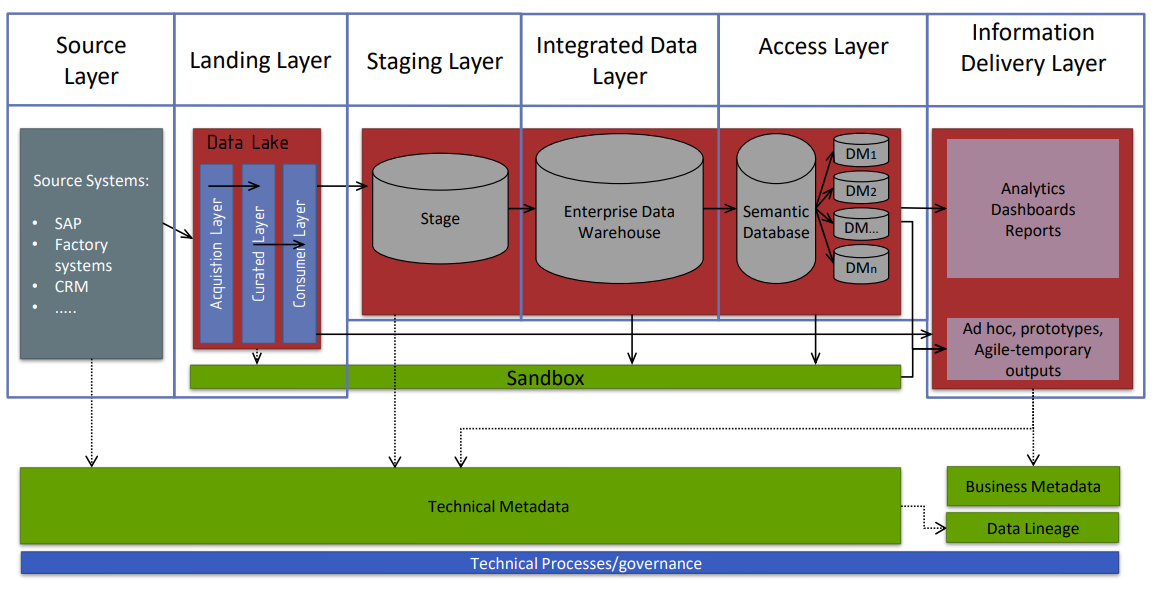
\includegraphics[width=\textwidth]{DP-obrazky/DWH_architektura.png}
    \caption{Model Datového skladu, přednáška MI-DWH \cite{EDW2}}
    \label{fig:DWH_Model}
\end{figure}



\begin{description}
    \item[Source Layer] slouží k napojení zdrojových systémů pro automatizaci získávání zdrojových dat. V mém případě jsou zdrojová data nahrána z CSV souborů, které jsou buď ručně získány ze zdrojů, či v případě Google Trends pomocí vytvořeného Python skriptu využívajícího k tomuto učelu sloužící API. Tato vrstva je tedy v mém případě vynechána, neboť majorita využitých datových souboru byla získána ručně. \cite{EDW-C1}
    
    \item[Landing layer] je volitelná vrstva a slouží k případné transformaci dat před samotným nahráním do Stage databáze. V mém případě se jedná zejména o sjednocení názvů zemí, kterého bylo dosažena pomocí dalšího mnou vytvořeného Python skriptu. Dále se jedná pouze o drobné úpravy týkající se špatného formátu datového souboru, které neumožňuje automatické zpracování, jako například vložené řádky textu, který neodpovídá hlavičce, nebo chybějící oddělovače. \cite{EDW-C1}
    
    \item[Stage Layer] obsahuje databázi, do které jsou nahrávány surová data z datových exportů. Slouží zejména pro validaci dat před nahráním do Integrated Data Layer. Tuto část využívám pro kontrolu dat a pro jednodušší následnou manipulaci a čištění pomocí ETL procesů (Extract, Transform, Load) při nahrávání do další vrstvy. Další výhodou je i to, že po nahrání do Stage databáze mají všechna data sjednocený datový typ, což je potřeba pro jejich vzájemné párování a porovnávání.  \cite{EDW-C1}
    
    \item[Integrated Data Layer], jinak také známý jako Target.  Do této databáze s jednotným datovým modelem, který popisuje všechny entity zde uložené, se ukládají transformovaná data ze Stage vrstvy. Tato data jsou dle potřeby historizována a jsou zde využity technické sloupce, aby bylo možné jednotlivé záznamy jednoznačně odlišit. Toto je srdce celého datového skladu, ve kterém se všechna potřebná data soustředí, a tedy je tato vrstva implementována i v mém případě.  \cite{EDW-C1}
    
    \item[Access Layer] obsahuje jednotlivá datová tržiště, která mají napočítána často agregovaná data na základě specifických požadavků. Často jsou obohacena o sémantickou databází, která zaručuje "jednotnou pravdu" v datových tržištích. V mém případě je vytvořeno datové tržiště a sémantická vrstva je vypuštěna. Jednotná pravda je zde zajištěna pomocí skriptu, který sjednocuje názvy zemí, a také pomocí jednotného formátu datumu. Díky tomu jsou veškeré společné sloupce jednotné.  \cite{EDW-C1}
    
    \item[Information Delivery Layer] slouží pro přístup k datům ze strany uživatele. Pro tyto potřeby se využívají různé reportovací, analytické, prediktivní nástroje a modely. Opět pro mé potřeby samozřejmostí a je využito reportovacího systému ve formě dashboardu, který je zprostředkován pomocí Power BI a následně zveřejněn na webových stránkách.  \cite{EDW-C1}
\end{description}


\section{Extract, Transform, Load (ETL)}

Jak již název napovídá, jedná se o tři procesy, které slouží pro kopírování dat z jednoho či více zdrojů do cílového úložiště v jiném kontextu a formě. Tyto procesy se mohou provádět ručně nebo automaticky pomocí k tomu určených programů (Power Query, Pentaho DI,...). Cílem procesů je převést data do podoby, v které je chceme dále uchovávat. Tato podoba bývá vhodná pro analytické účely a nemusí zde být zajištěna třetí normální forma. Dále pomáhají udržovat čistotu a datovou kvalitu, díky čemuž se ukládají jen data důležitá pro další analýzy a BI. 

Někdy se také používají procesy v podobě ELT, kdy se data transformují až po nahrání do finálního úložiště či jejich kombinace v závislosti na situaci. ETL/ELT procesy by měly mít následující vlastnosti: \cite{EDW4}

\begin{itemize}
    \item Transakční zpracování potřebné pro správnou komunikaci s databázovými systémy a jejich transakcemi (transakce proběhne pouze jako celek, jinak je celá rollbacknutá).
    \item Kontrola datové kvality aspoň na základní úrovni.
    \item Zpracování výjimek - musí umět odchytit a vyhodnotit výjimku, která nastane v průběhu zpracování.
    \item Idempotentnost - opakované provedení procesů vede ke stejnému výstupu.
    \item Logování - pro přehlednější kontrolu průběhu a zpracování informací při nastalých chybách.
\end{itemize}


\section{Historizace dat}
Na rozdíl od klasických databází, kde nás zajímá pouze aktuální stav dat, v datových skladech je důležité, i jak data vypadala v historii, aby mohly být jejich změny analyzovány a na jejich základě být vytvářeny predikční a statistické modely.

Protože ne u všech dat je potřeba držet plnou historizaci, tak při práci s datovými sklady existují tři úrovně historizace, které se dnes nejběžněji využívají: \cite{EDW3}

\begin{description}
    \item[SD0] - Zachovává se pouze stávající hodnota, pokud přijde do databáze pokus o uložení dat pro daný identifikátor a jinými daty, jedná se nejpravděpodobněji o chybu. Operace INSERT.
    \item[SD1] - Přepsání stávající hodnoty za novou. Udržují se pouze aktuální data. Operace INSERT, UPDATE.
    \item[SD2] - Udržování úplné historie, kdy je pro každý nový záznam vytvořena nová kopie s unikátním technickým klíčem a časovými záznamy doby platnosti. Protože tento typ historizace je nejdůležitější, neboť se udržuje kompletní verzovaná historie, tak pro lepší předsstavu je na obrázku 4.2 ukázka záznamu, kde se pro studenta s ID 2529 a SK 5 změní stav o akademických titulech. Je tedy vytvořen nový záznam s identickým SK a id\_student a každému záznamu je přiřazen unikátní T\_ID. Dále jsou zde uloženy hodnoty o období platnosti VALID\_FROM a VALID\_TO. 
\end{description}

\begin{figure}
    \centering
    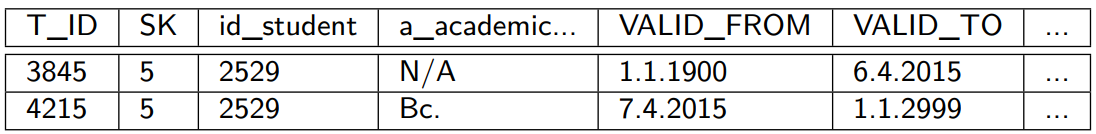
\includegraphics[width=\textwidth]{DP-obrazky/SD2.png}
    \caption{Ukázka záznamu s typem historizace SD2 \cite{EDW3}}
    \label{fig:SD2}
\end{figure}


\section{Dimenzionální databáze}
Tyto databáze se nejčastěji využívají v datových skladech v části zvané datamart. Pro jejich implementaci lze využít pouze náhledy do hlavní centrální databáze (targetu) nebo pro ně vytvořit vlastní tabulky. Tyto databáze jsou uzpůsobeny pro potřebnou analýzu daných problémů a každý samotný datamart by měl odpovídat na určitou problematiku  či skupině souvisejících problémů. Proto také často obsahují již agregovaná data, která následně urychlují odpovědi na případné dotazy ze strany uživatele.

Díky tomu, že tyto databáze mají různé dimenze náhledu, můžeme zkoumat dané problémy s proměnlivou hloubkou a zaměřením. Nejčastějšími dimenzemi jsou časová, polohová, produktová či kategorická, což souvisí s jejich primárním účelem podpořit business společnosti, jež tyto sklady používá, a je pro ni tedy zásadní zkoumat úspěch jejich prodejen a obchodovaného portfolia. 

Nejčastější podoby dimenzionálních tabulek bývají buď hvězda, kdy jsou na faktovou tabulku přímo vázány všechny dimenze, a nebo vločka, kdy mohou dimenzionální tabulky mít podtabulky, do kterých se větví. Zatímco hvězda je jednodušší z hlediska implementace a vzájemného propojení, díky maximální hloubce propojení rovné jedné, tak vločka mnohem lépe podporuje následné úpravy a přidávání dalších kategorií a nové dělení, které vede v případě vločky pouze k připojení nové poddimenze, kdežto u hvězdy je třeba předělat již existující dimenzionální tabulku.  

\begin{figure}
    \centering
    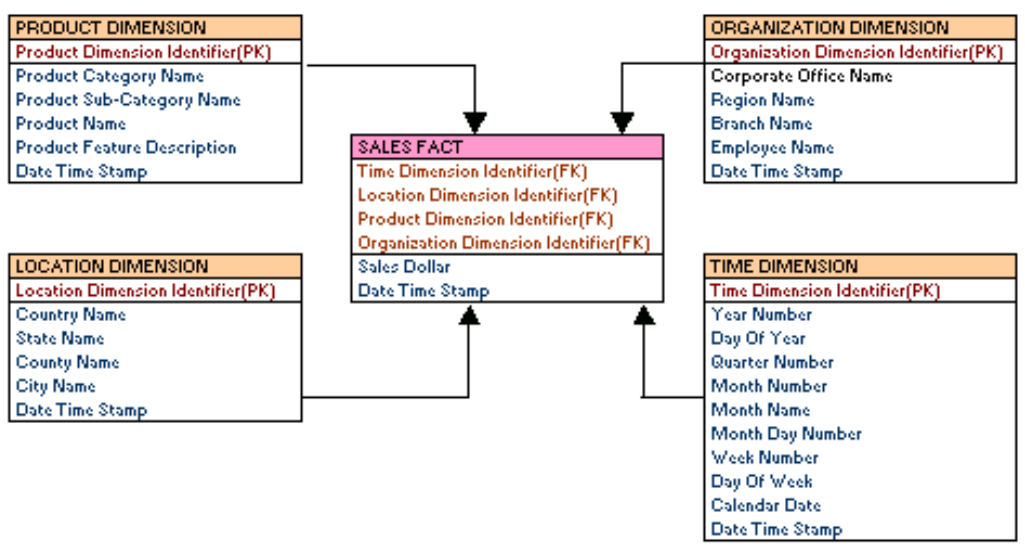
\includegraphics[width=\textwidth]{DP-obrazky/DD_hvezda.png}
    \caption{Příklad schématu dimenzionální databáze v schématu hvězdy. Z cvičení MI-DWH. \cite{EDW5}}
    \label{fig:Dim_Hvězda}
\end{figure}



\begin{figure}
    \centering
    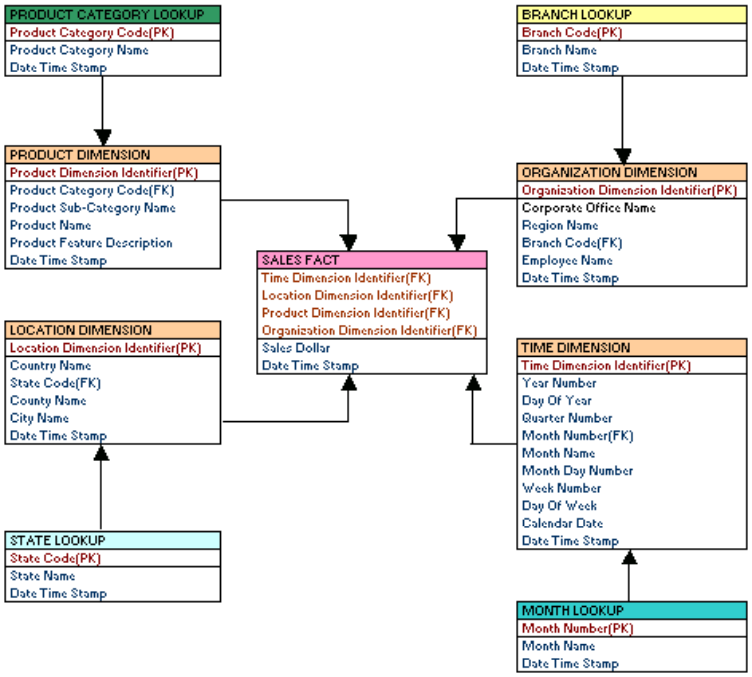
\includegraphics[width=\textwidth]{DP-obrazky/DD_vlocka.png}
    \caption{Příklad schématu dimenzionální databáze v schématu vločky. Z cvičení MI-DWH. \cite{EDW5}}
    \label{fig:Dim_vločka}
\end{figure}



Centrem všeho je faktová tabulka, která je postavena tak, aby odpovídala na určitý dotaz. Tato tabulka na sebe následně váže ostatní dimenzionální tabulky, které ji umožní měnit náhledy na danou problematiku v osách různých dimenzí. Například se můžeme v našem případě podívat na celosvětovou plodnost aktuálně, ale také pouze na plodnost v Evropě či Austrálii, a to v letech 1990 - 2000. 

Faktová tabulka dále často obsahuje předpočítané proměnné, které jsou pro dané položené dotazy využívaný, aby se tak šetřil čas, který by jejich okamžitý výpočet ze surových dat trval. \cite{EDW5}

\section{Dashboard}

Jedná se o specializované programy, které jsou určeny pro práci s datamarty. Slouží k vizualizaci daných analytických sad a k živé práci s různými dimenzemi u daných faktů. Jsou vhodné pro svou výtečnou prezentaci za použití vhodných vizualizačních prostředků, díky nimž je zajištěna dobrá čitelnost. Pomáhá zodpovídat otázky a podporuje analýzu a rozhodování. Také nám může pomoc utvářen nové pohledy na danou problematiku a pomáhá prezentovat výsledky druhým.

Vizualizace by tedy měla být přehledná a snadno čitelná, aby byly důležité výsledky a hodnoty uživatelům přímo na očích. Tvůrce by se měl vyvarovat složitých a rozptylujících prvků a jiného tzv. šumu. \cite{EDW5})
Nejčastější způsoby vizualizace jsou následující prvky:

\begin{description}
    \item[Bar chart] - Sloupce jsou ideální pro reprezentaci míry, a jsou tedy vhodné pro porovnávání kategorických dat.
    
    \item[Line chart]  - Vhodné pro zobrazení změn v průběhu času, pomocí spojnice sledujeme trendy.
    
    \item[Scatter plot] - Užitečné pro zobrazení vztahu mezi dvěma proměnnými.
    \item[Heatmap] - Tabulka, která využívá barvu ke zvýraznění rozdílů mezi jednotlivými hodnotami.

    \item[Tabulka] - Je vhodná pro zobrazení přesných hodnot.
    \cite{EDW5}
\end{description}

\begin{figure}
    \centering
    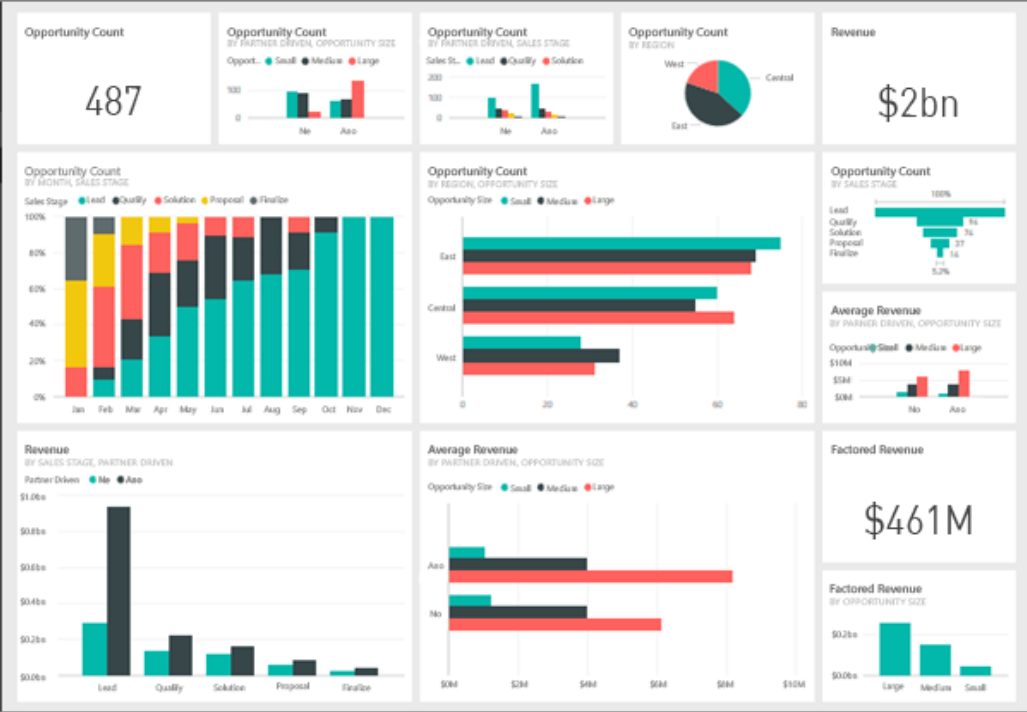
\includegraphics[width=\textwidth]{DP-obrazky/dashboard_rnd.png}
    \caption{Dashboard v Power BI. Zdroj prezentace MI-DWH \cite{EDW5}}
    \label{fig:Dashboard_př}
\end{figure}




\section{Business intelligence}

Business intelligence je sada procesů, know-how, aplikací a technologií, které slouží pro optimalizaci procesů, umožňují získat přehled o dění v instituci a vytváří určité výhody oproti konkurenčním institucím.

Jedná se tedy o celkovou disciplínu, která využívá různé technologie a principy a pomocí nich a analytických metod dochází k závěrům, které mohou sloužit pro optimalizaci a vylepšení každodenních procesů. V případě této práce zkoumáme socioekonomické aspekty a vlivy na TFR, kdy po následné analýze různých faktorů můžeme dojit k jisté optimalizaci procesů, jenž s danými faktory souvisí, a tím i přispět k následnému budoucímu růstu úhrnné plodnosti i třeba jen o malé, leč významné hodnoty.

Ve spojení s BI se zkoumané problémy řeší za pomocí KPI (key performance indicator = klíčové ukazatele výkonnosti). Tyto ukazatele nám mají referovat míru vlivu a úspěšnosti v dané zkoumání části. V našem případě mohou být takovými hodnotami, které nám ukazují míru vlivu daného faktoru na TFR, například základní statistické hodnoty, jako jsou například míra korelace, či p-hodnota a s ní související výsledky testů hypotéz. \cite{EDW1}

\chapter{Návrh datového skladu}

Cílem této kapitoly je seznámit čtenáře s návrhem a podobou datového skladu, který je využit pro uložení, vhodné transformování a následnou analýzu všech vybraných datových sad. 

Pro potřeby tvorby všech procesů potřebných k vývoji byly využity nástroje k tomu určeny. Tyto nástroje byly získány v rámci školní licence či v podobě freewaru, který má samozřejmě své nedostatky, ale v rámci této práce je zcela dostačující.

Prvním nástrojem je \textbf{Enterprise Architect} \cite{EA}, který je velmi oblíbený jak při práci během našeho studia, tak i v mnohých společnostech. Tento nástroj je skvělý pro vytváření všech typů modelů a pro tuto práci byl využit pro návrh databázových modelů. Díky jeho funkci generování DDL souborů byly následně z modelů vytvořeny SQL skripty, které mají za úkol připravit v určené databázi všechny potřebné tabulky, do nichž se budou následně automaticky nahrávat veškeré potřebné soubory a data.

Databaze je postavena na \textbf{PostgreSQL} \cite{postgres} a je spravována v rámci vývoje v aplikaci \textbf{Postbird} \cite{postbird}, která nabízí všechny služby nutné pro správu všech databází potřebných pro tuto práci. 

Všechny automatické ETL procesy byly zpracovány pomocí \textbf{Pentaho Data Integration} \cite{pentaho}, což je freeware, který je určen pro automatizaci zpracování datových sad. Je skvělý pro načítání surových dat a jejich následné vkládání do databáze a samozřejmě jejich transformaci do podoby vhodné pro následnou analýzu. Protože se jedná o freeware, má samozřejmě i jisté nedostatky, které byly řešeny různými kličkami a případně bylo využito možnosti spouštět i vlastni Python skripty, které jsem pro potřeby další transformace a sjednocení dat vytvořil.

Samotné python skripty jsem vyvíjel ve \textbf{Visual Studio Code} \cite{VSC}, což je skvelé IDE pro práci ve všech možných programovacích jazycích. Pro své potřeby jsem  s využitím knihovny \textbf{pytrends} \cite{pytrends} vytvořil skripty pro automatické stahování dat z Google Trends, který je jedním z mých důležitých datových zdrojů. Dále jsem využil knihovny \textbf{country\_converter} \cite{CC}, kterou jsem potřeboval pro sjednocení názvů zemí, aby bylo možné dané sady snadno strojově porovnávat (Neboť “Czechia” a “Czech Republic” je pro SQL dotaz inner join i samotnou relaci problém).

Součástí skriptu je i ověření stacionarity datových sad, k čemuž slouží knihovna \textbf{statsmodels} \cite{stat}, z níž využívám funkce \textit{adfuller} a \textit{kpss}. Pokud je následně u datového souboru potvrzena nestacionarita, jsou jeho hodnoty diferencovány pomocí knihovny  \textbf{numpy} \cite{numpy}. V poslední řadě nelze zapomenout na knihovnu \textbf{Pandas} \cite{pandas}, která obsahuje nástroje pro práci s Dataframy, jež jsou vhodné pro ukládání těchto statistických dat, a také funkce pro načítání a ukládání csv souborů.

Pro samotnou analýzu dat a jejich vhodnou vizualizaci jsem zvolil nástroj \textbf{Power BI} \cite{powerbi}, jenž je součástí \textit{Microsoft Office 365}, který máme k dispozici v rámci školní licence. V tomto nástroji je možné vytvářet libovolné vizualizace na datech připojených jak ze souborů, tak z databází. Také nabízí šikovné možnosti filtrování dat, které se zobrazují a díky vlastnímu programovacímu jazyku \textit{Power Query M} lze vytvářet i vlastní míry, pokud si uživatel nevystačí s těmi, které jsou již v rámci nástroje předpřipravený. Také obsahuje možnost vytvářet vlastní vizualizace a výpočty na datech pomocí jazyků \textit{R} a \textit{Python}, čehož bylo také využito pro kompletní zobrazení všech potřebných statistických veličin.

\section{Sběr dat}

Data byla získávána z několika zdrojů ve formátu csv. Všechny tyto soubory obsahovaly pro mou následnou analýzu stěžejní hodnoty, jako je země, rok a hodnota. Přestože ne všechny sady obsahovaly veškerá data pro všechny země či časové úseky, pro samotnou statistickou hodnotu to nemělo zásadní vliv, neboť takové hodnoty nebyly na sebe jednoduše napárovány a nebyly tak v následné analýze zahrnuty. To ovšem nevadí, neboť se používala data ze všech dostupných zemí, a tak byl daný vzorek velmi bohatý. 

Jedním z nich byl již výše zmíněný \textbf{Google Trends} \cite{google}, z kterého byla data stažena pomocí vytvořeného Python skriptu. Z důvodu omezení ze strany Googlu, kdy při větším množství dotazů z jedné IP adresy docházelo k přerušení spojení a konci stahování dané sady, jsem do kódu vložil sleep, který měl tento problém eliminovat, ale ani tak nebylo možné tyto velké datové sady stáhnout naráz. Proto jsem je stahoval po částech, které jsem ukládal do samotných csv souborů, které jsem následné pomocí dalšího mnou vytvořeného skriptu sloučil do jediného souboru. 

Google Trends poskytuje svá normalizovaná data o vyhledávání určitých témat a frází ze všech dostupných zemí od roku 2004. Normalizovaná jsou tak, že misto surových hodnot jsou jednotlivé hledání v daných zemích hodnoceny ve škále od jedné do sta. Časově jsou data poskytována za každý měsíc, takže aby odpovídala ostatním veličinám, které jsou sbírány v roční frekvenci, byla tato data zprůměrována, a tím byla získána finální roční hodnota.

Druhým významným zdrojem je \textbf{World Bank Group} \cite{worldbank}, která pod sebou sdružuje pět organizací, jež mají za cíl obnovu a rozvoj zejména v rozvojových zemích. Tato skupina vznikla v roce 1944 a postupně se rozšiřovala o další dílčí organizace, které jsou nyní její součástí. Sdružuje 189 členských států a její součástí je i Development Data Group, která spravuje databáze shromažďující statistická data členských zemí. To ve výsledku dává bohatou kolekci dat s dostupnými indikátory pro široké územní i časové spektrum. Díky tomu, že jsou tyto data volně dostupná, jsou také vhodným zdrojem získávání potřebných datových sad. 

Posledním zdrojem je \textbf{Our World in Data} \cite{OWD}, což je výsledek spolupráce mezi University of Oxford a neziskovou organizací \textit{Global Change Data Lab}. Cílem toho spojenectví je zmapovat, jak se v globálním měřítku mění podmínky pro žití, životní prostředí a další důležité ukazatelé, které ovlivňují jak jednotlivé regiony, tak celý svět. K tomu využívá kromě vlastních dat a výzkumů, která jsou vytvořena ve spolupráci s \textit{Oxfordskou Univerzitou} a dalšími dobrovolnými pracovníky, také data a práce, které vytvářejí jednotlivé instituce v daných zemích, a nejsou tak široké veřejnosti dostupné.

% Please add the following required packages to your document preamble:
% \usepackage{booktabs}
% \usepackage{graphicx}
\begin{table}[h]
\caption{Tabulka datových sad s jejich zdroji a základními parametry dat v jednotlivých sadách.}
\resizebox{\textwidth}{!}{%
\begin{tabular}{@{}ccccc@{}}
\toprule
\textbf{Název veličiny} &
  \textbf{Zdroj} &
  \textbf{Počet zemí} &
  \textbf{Časový rozsah} &
  \textbf{Jednotka} \\ \midrule
\multicolumn{1}{|c|}{TFR \cite{fr}} &
  \multicolumn{1}{c|}{Our World in Data} &
  \multicolumn{1}{c|}{198} &
  \multicolumn{1}{c|}{1950-2018} &
  \multicolumn{1}{c|}{num. of kids per woman} \\ \midrule
\multicolumn{1}{|c|}{Country \cite{country}} &
  \multicolumn{1}{c|}{World Bank} &
  \multicolumn{1}{c|}{209} &
  \multicolumn{1}{c|}{-} &
  \multicolumn{1}{c|}{country} \\ \midrule
\multicolumn{1}{|c|}{BMI female \cite{BMI}} &
  \multicolumn{1}{c|}{Our World in Data} &
  \multicolumn{1}{c|}{199} &
  \multicolumn{1}{c|}{1975-2016} &
  \multicolumn{1}{c|}{kg/m2} \\ \midrule
\multicolumn{1}{|c|}{Cat} &
  \multicolumn{1}{c|}{Google Trends} &
  \multicolumn{1}{c|}{222} &
  \multicolumn{1}{c|}{2004-2020} &
  \multicolumn{1}{c|}{mean year score} \\ \midrule
\multicolumn{1}{|c|}{Disasters \cite{disasters}} &
  \multicolumn{1}{c|}{Our World in Data} &
  \multicolumn{1}{c|}{203} &
  \multicolumn{1}{c|}{1990-2019} &
  \multicolumn{1}{c|}{num. of death per 100 000 inhabits} \\ \midrule
\multicolumn{1}{|c|}{Dog} &
  \multicolumn{1}{c|}{Google Trends} &
  \multicolumn{1}{c|}{186} &
  \multicolumn{1}{c|}{2004-2020} &
  \multicolumn{1}{c|}{mean year score} \\ \midrule
\multicolumn{1}{|c|}{Female labour \cite{labor}} &
  \multicolumn{1}{c|}{World Bank} &
  \multicolumn{1}{c|}{215} &
  \multicolumn{1}{c|}{1960-2021} &
  \multicolumn{1}{c|}{\%} \\ \midrule
\multicolumn{1}{|c|}{Infertility} &
  \multicolumn{1}{c|}{Google Trends} &
  \multicolumn{1}{c|}{133} &
  \multicolumn{1}{c|}{2004-2020} &
  \multicolumn{1}{c|}{mean year score} \\ \midrule
\multicolumn{1}{|c|}{IVF} &
  \multicolumn{1}{c|}{Google Trends} &
  \multicolumn{1}{c|}{155} &
  \multicolumn{1}{c|}{2004-2020} &
  \multicolumn{1}{c|}{mean year score} \\ \midrule
\multicolumn{1}{|c|}{P90vsP10 \cite{p90}} &
  \multicolumn{1}{c|}{Our World in Data} &
  \multicolumn{1}{c|}{161} &
  \multicolumn{1}{c|}{1981-2017} &
  \multicolumn{1}{c|}{-} \\ \midrule
\multicolumn{1}{|c|}{Schooling \cite{schooling}} &
  \multicolumn{1}{c|}{Our World in Data} &
  \multicolumn{1}{c|}{192} &
  \multicolumn{1}{c|}{1870-2017} &
  \multicolumn{1}{c|}{years} \\ \midrule
\multicolumn{1}{|c|}{Urbanization \cite{urban}} &
  \multicolumn{1}{c|}{Our World in Data} &
  \multicolumn{1}{c|}{211} &
  \multicolumn{1}{c|}{1960-2020} &
  \multicolumn{1}{c|}{-} \\ \midrule
\multicolumn{1}{|c|}{Working hours \cite{working hours}} &
  \multicolumn{1}{c|}{Our World in Data} &
  \multicolumn{1}{c|}{70} &
  \multicolumn{1}{c|}{1870-2017} &
  \multicolumn{1}{c|}{h} \\ \midrule\bottomrule
\end{tabular}%
}
\end{table}

\section{Stage}

Do první databázové části se nahrávají data v surové podobě. V tomto případě se jedná o soubory v podobě, v které byly staženy. V případě dat získaných pomocí skriptu z Google Trends, jenž byl za tímto účelem vytvořen, jsou již data stahována v potřebné podobě a při slučování dílčích souborů jsou zároveň již sjednoceny názvy zemí. 

Databáze se před každým nahráním vyčistí, aby byla udržována vždy jen aktuální iterace a samotná data se zbytečně neduplikovala. Pro každý soubor je vytvořena samostatná tabulka, která obsahuje všechny hodnoty tak, jak jsou v nahraném souboru.

Dále se zde nachází pomocné tabulky, kde se uchovávají dočasná data pro další zpracování pomocí skriptu či následné nahrání do Target databáze po transformaci.

\begin{figure}
    \centering
    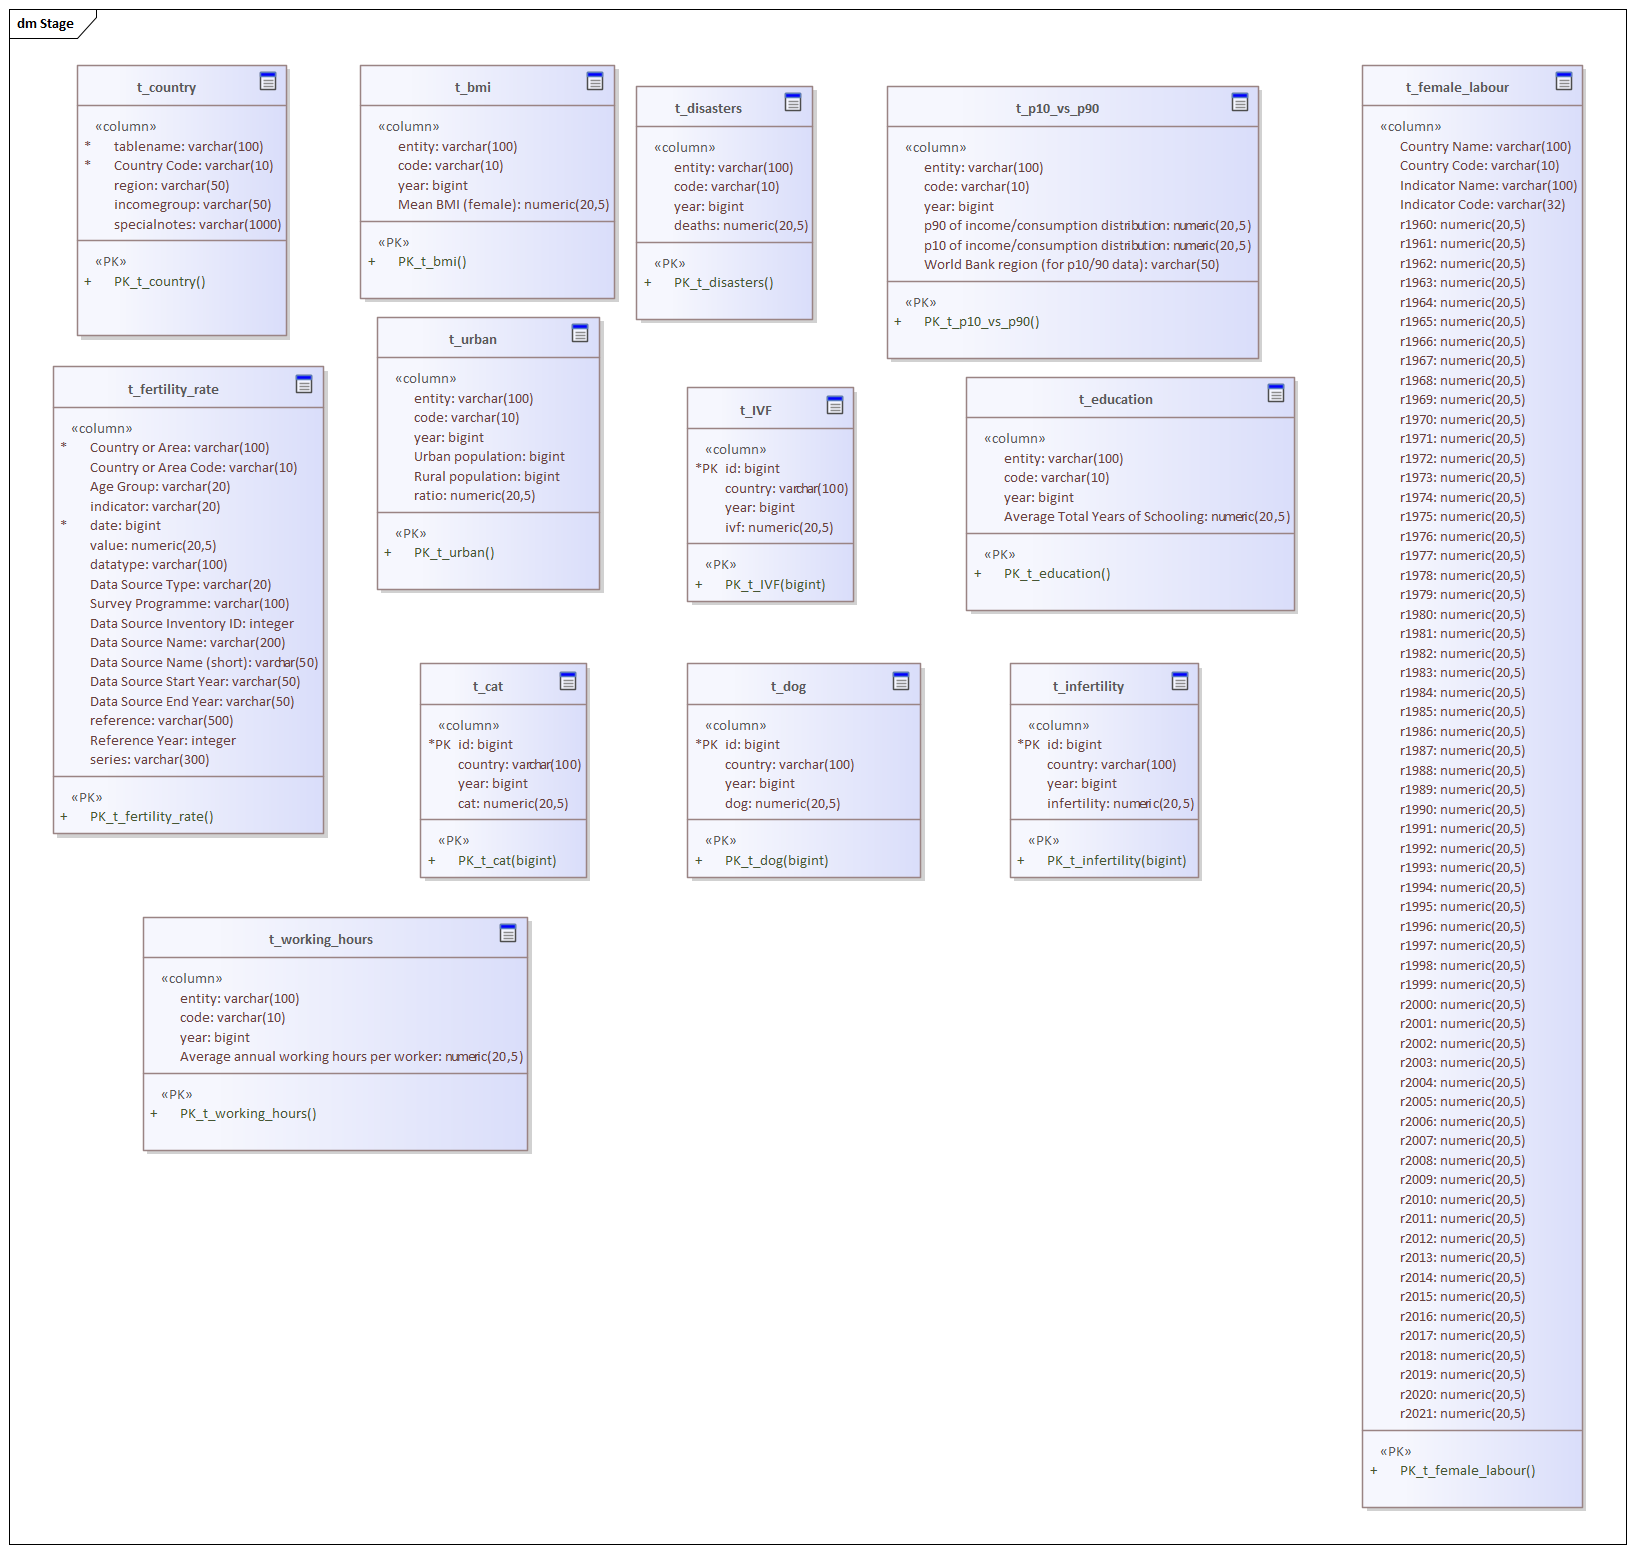
\includegraphics[width=\textwidth]{DP-obrazky/Stage.png}
    \caption{Obrázek modelu Stage databáze v programu Enterprise Architect.}
    \label{fig:Stage_model}
\end{figure}

Logický model byl vytvořen v Enterprise Architectu a je tvořen pro PostgreSQL databázi. Pro ni je i generovaný samotný kód pro vytvoření databáze a tabulek, jež obsahuje, a to přímo z již výše zmíněného nástroje.

Když je databáze správně vytvořená a spárována s nástrojem Pentaho Data Integration, lze pak soubory nahrát automaticky spuštěním Jobu Stage. Ten vždy dané tabulky vyčistí a následně tam nahraje nová data.

\begin{figure}
    \centering
    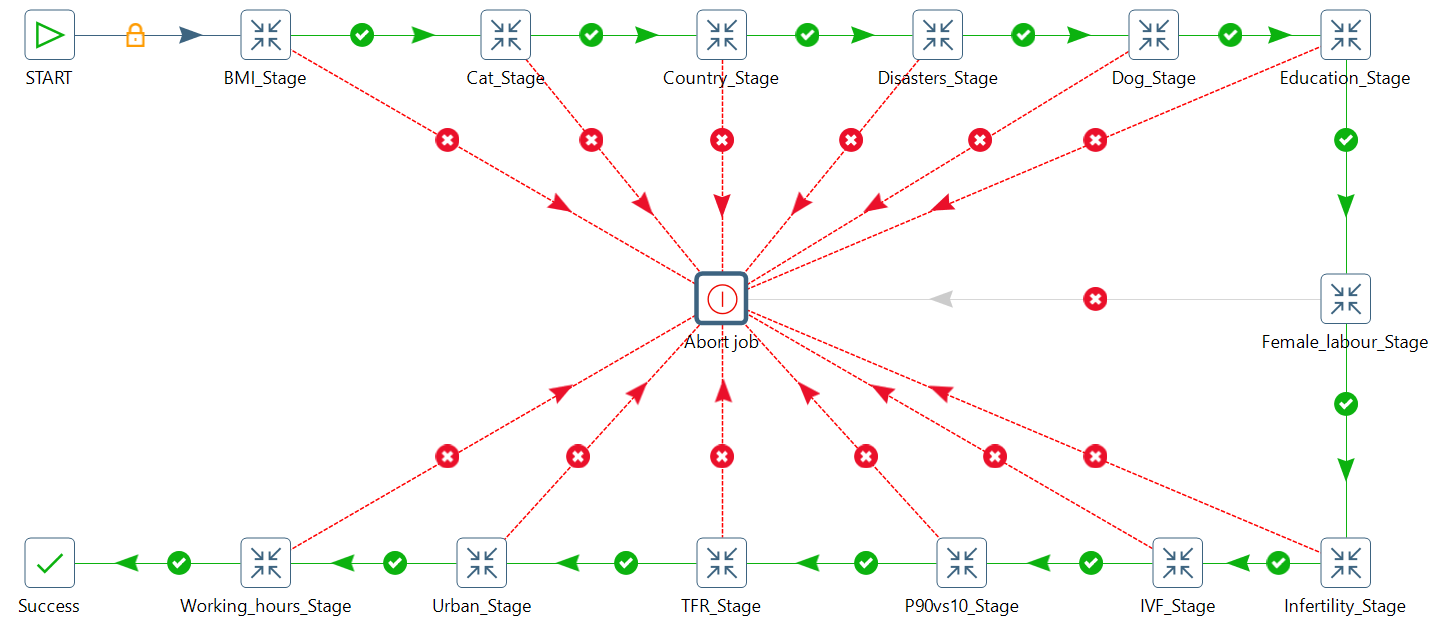
\includegraphics[width=\textwidth]{DP-obrazky/Stage_Pentaho.png}
    \caption{Pentaho Stage Job se všemi transakcemi, které se postupně dle modelu spouští.}
    \label{fig:Stage_ETL}
\end{figure}

\section{Target}

Databáze Targetu je srdcem celého datového skladu, zde se ukládá a historizuje vše důležité. Proto v průběhu ETL procesů dochází k čištění a transformaci dat tak, aby byla následná práce s nimi co nejefektivnější. Proto zde bylo spoustu sloupců zahozeno a nebo transformováno do jiné, pro naši analýzu vhodnější, podoby. Všechny tyto transformační procesy jsou, při správném nastavení databází a cest v proměnných prostředí v nástroji Pentaho DI, zcela automatické a proběhnou při tvorbě samotného datového skladu. 

Všechny transakce, které slouží k předpřipravení všech dat pro transformaci pomocí python skriptu, jsou součástí Pentaho Jobu Transform. Ten data pročistí a případně upraví do vhodné podoby, aby na nich následně mohl být spuštěn daný skript, který má za úkol sjednotit názvy všech zemí a ověřit stacionaritu dat v těchto časových řadách. Pokud jsou data nestacionární, je na nich následně provedena diferenciace, aby byla stacionarita zajištěna. Veškeré mezikroky v transformaci se ukládají do CSV souborů v příslušných složkách, díky čemuž jsou veškeré mezikroky uloženy a je tedy možné sledovat a ověřovat dané postupy.

\begin{figure}
    \centering
    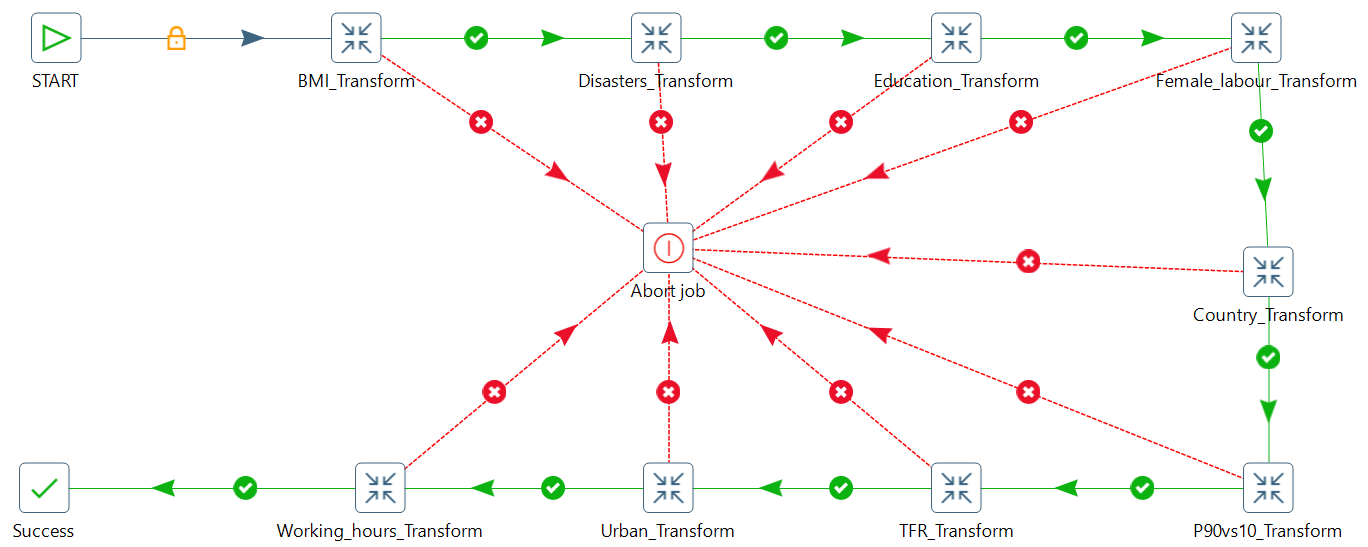
\includegraphics[width=\textwidth]{DP-obrazky/Transform.png}
    \caption{Pentaho Transform Job se všemi transakcemi, které se postupně dle modelu spouští.}
    \label{fig:Transform_ETL}
\end{figure}

Při transformaci byly ke každé tabulce přidaný čtyři technické sloupce, které jsou potřebné pro správnou historizaci dat. Jedná se o:

\begin{itemize}
    \item TK - technický klíč, který funguje jako nový umělý identifikátor
    \item version - tento sloupec nám udává, o kolikátou verzi dané tabulky v rámci historizace se jedná
    \item Date\_from - timestamp, který udává, od jakého data je daná verze tabulky platná
    \item Date\_to - timestamp, který udává, do kdy je daná verze tabulky platná
\end{itemize}

\begin{figure}
    \centering
    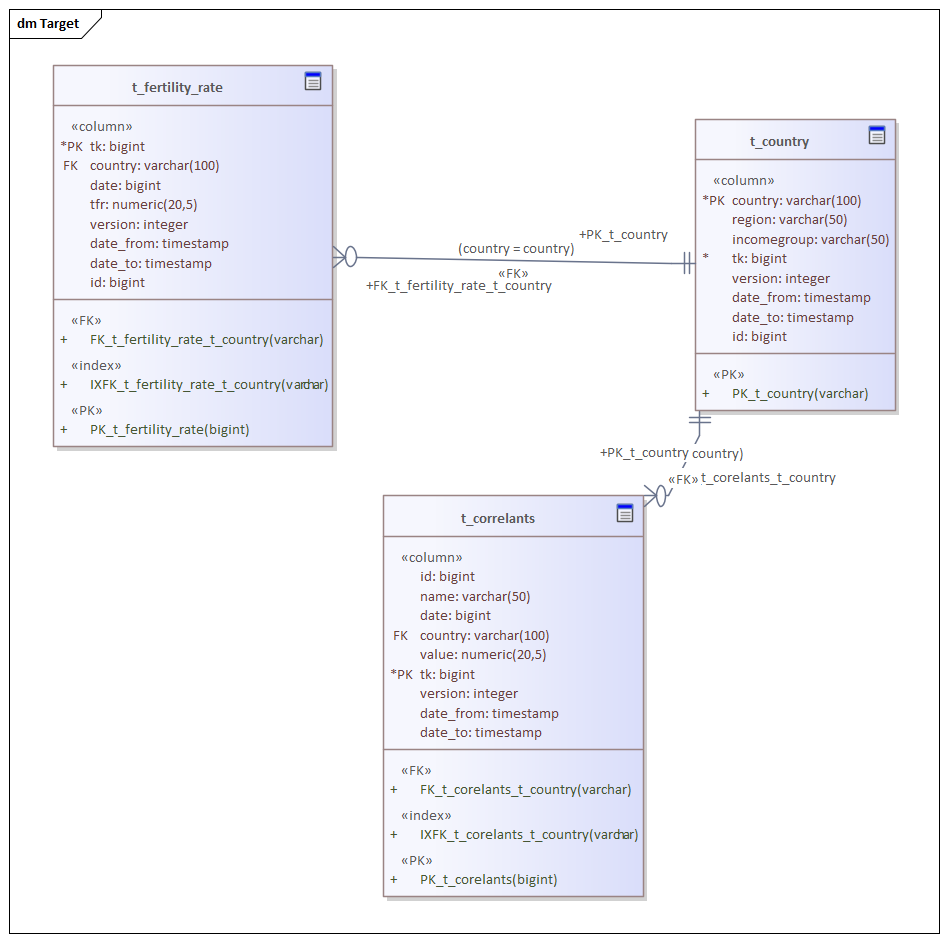
\includegraphics[width=\textwidth]{DP-obrazky/Target.png}
    \caption{Obrázek modelu Target databáze v programu Enterprise Architect.}
    \label{fig:Target_model}
\end{figure}

Samotná databáze byla oproti Stage zjednodušená na pouhé tři tabulky, kdy jedna je určena pro TFR (t\_fertility\_rate). Ta obsahuje následující sloupce vyjma těch technických:

\begin{itemize}
    \item Country - pro polohovou lokalizaci dané veličiny. Je v relaci s tabulkou t\_country, díky čemuž lze hodnoty filtrovat dále dle regionů a příjmů
    \item Date - pro určení roku, pro který je daná hodnota platná
    \item tfr - stacionární (diferencovaná) hodnota TFR pro danou zemi v daný rok
\end{itemize}


Další tabulkou je pomocná tabulka t\_country, díky níž lze lépe pracovat s polohovým určením a kromě jednotlivých států lze dané země seskupovat i podle regionů a příjmových skupin, což může pomoc lépe sledovat jejich vzájemné vlastnosti pro určité veličiny.

\begin{itemize}
    \item Country - název země
    \item Region - jednotlivé země jsou sjednoceny do větších regionů, které mají krom geografie často společné i další vlastnosti
    \item Incomegroup - rozdělení zemí podle jejich ekonomického hodnocení a výkonnosti
\end{itemize}


Poslední tabulka t\_correlants obsahuje všechny ostatní veličiny, které chceme porovnávat vůči TFR, a má následující strukturu:

\begin{itemize}
    \item Country - stejně jako u TFR je vázána na t\_country a spolu s datem slouží k párování veličin
    \item Date - rok, pro který je daná veličina měřena
    \item Name - název veličiny, kterou chceme porovnávat s TFR. Je určen pro následné filtrování jednotlivých veličin v této tabulce
    \item Value - obsahuje samotnou hodnotu dané veličiny, u které je také po transformaci zajištěna stacionarita
\end{itemize}



I tato část má v Pentaho vytvořený Job s názvem Target, který slouží k nahrání dat z pomocných souborů. Dále také vytvoření všechny pomocné sloupce a nahraje data do Target databáze v historizované podobě. 

\begin{figure}
    \centering
    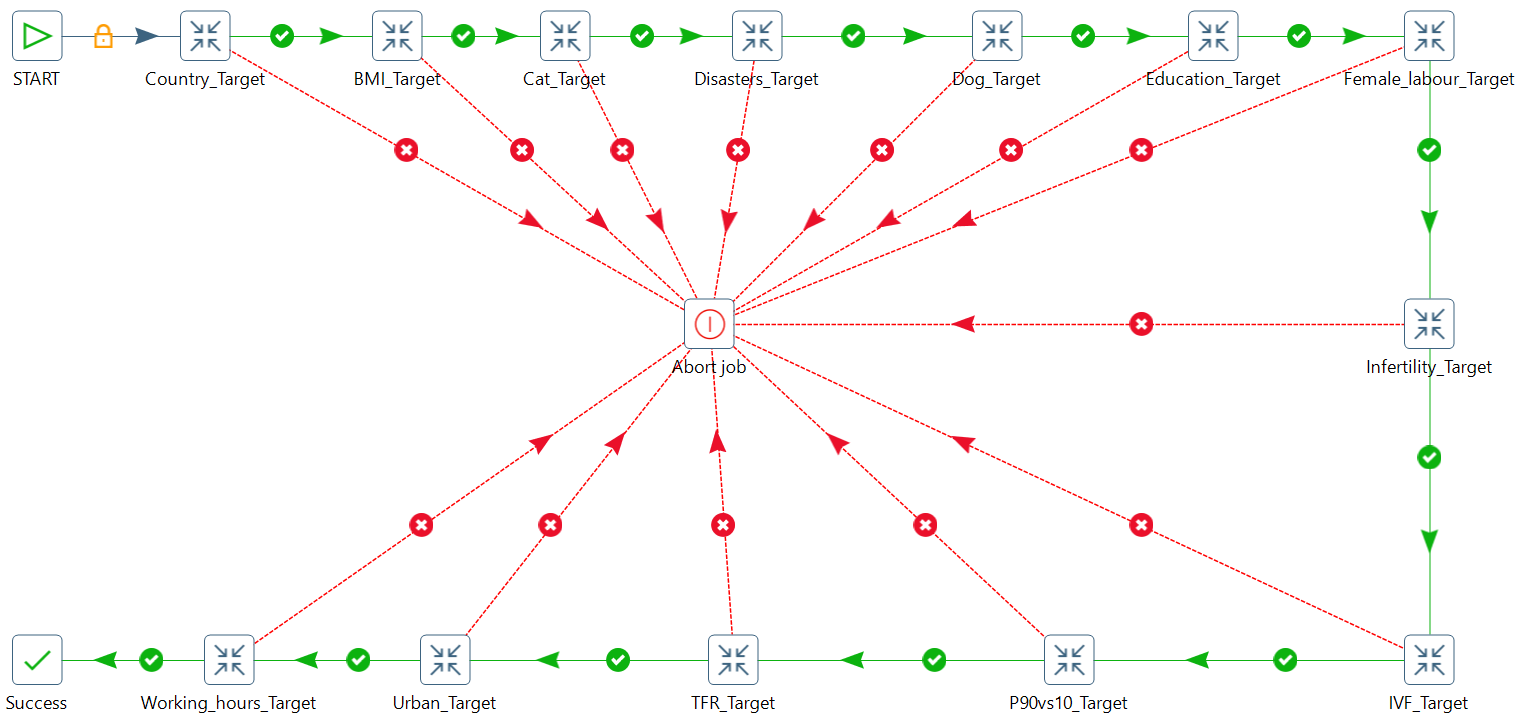
\includegraphics[width=\textwidth]{DP-obrazky/Target_Pentaho.png}
    \caption{Pentaho Target Job se všemi transakcemi, které se postupně dle modelu spouští.}
    \label{fig:Target_ETL}
\end{figure}

\section{Data Mart}

Tabulky dimenzionální databáze jsou vytvořeny pouze pohledy na samotnou Target databázi. Tím se ušetří prostor a pro potřeby naší analýzy je to zcela dostačující. Problém by nastal pouze ve chvíli, kdy by na tyto pohledy přicházelo v jednu chvíli velké množství dotazů a nebo by se původní tabulky neustále měnily, ale to není náš případ. 

\begin{figure}
    \centering
    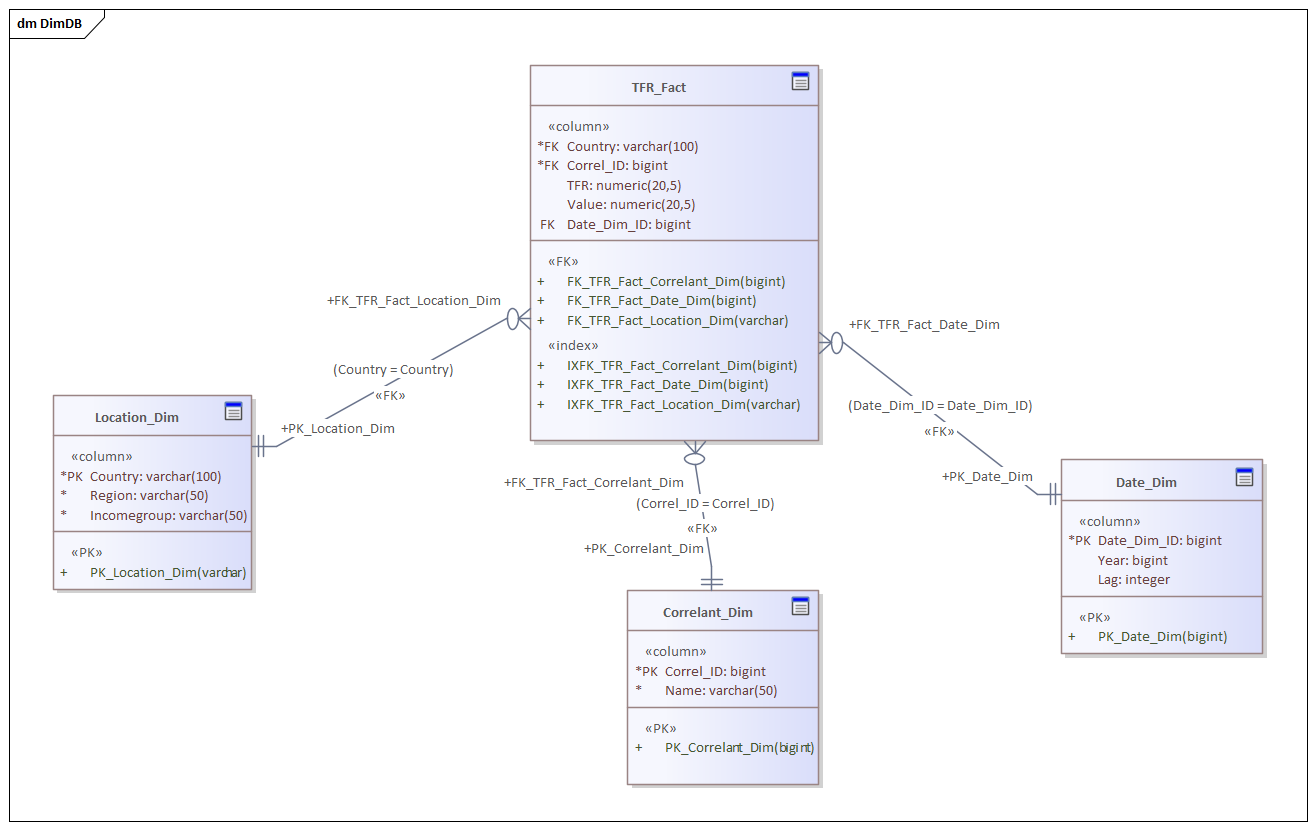
\includegraphics[width=\textwidth]{DP-obrazky/DimDB.png}
    \caption{Obrázek modelu dimenzionální databáze v programu Enterprise Architect.}
    \label{fig:DD_Model}
\end{figure}

Zde je vidět kompletní model dimenzionální databáze, kde hlavní tabulka krom odkazů na své dimenze obsahuje také vlastní hodnoty veličin, které jsou potřebné pro přímou analýzu.  
Jak je z modelu na obrázku 5.6 patrné, dimenze korelantů a datumu jsou velmi triviální, a tak je pro zjednodušení vhodné je při reálné tvorbě pohledů sloučit se samotnou tabulkou faktů. Toto sloučení je patrné z následujícího obrázku 5.7, který představuje již model v takové podobě, v jaké se nachází v dashboardu Power BI a z kterého se vytváří samotné vizuály.

Základní parametry, přes které je možné následně v samotném vizuálu dané hodnoty filtrovat, jsou v Location\_dim:

\begin{itemize}
    \item Country - lze sledovat hodnoty pro určitou zemi 
    \item Region - vybere skupinu zemí daného regionu, v kombinaci s volbou Country lze celkový výběr následně upravit
    \item Incomegroup - omezí země na danou skupinu dle jejich ekonomického hodnocení
\end{itemize}


Dále v Date\_dim jsou tyto dva parametry:

\begin{itemize}
    \item Date - pro určení přesného roku či časového úseku, pro který se data testují
    \item Lag - pro určení časového zpoždění sledované veličiny vůči hodnotě TFR

\end{itemize}


Posledním parametrem je pak \textbf{Name}, který nám umožňuje vybrat proměnnou, již chceme aktuálně porovnávat s TFR.

\begin{figure}[h]
    \centering
    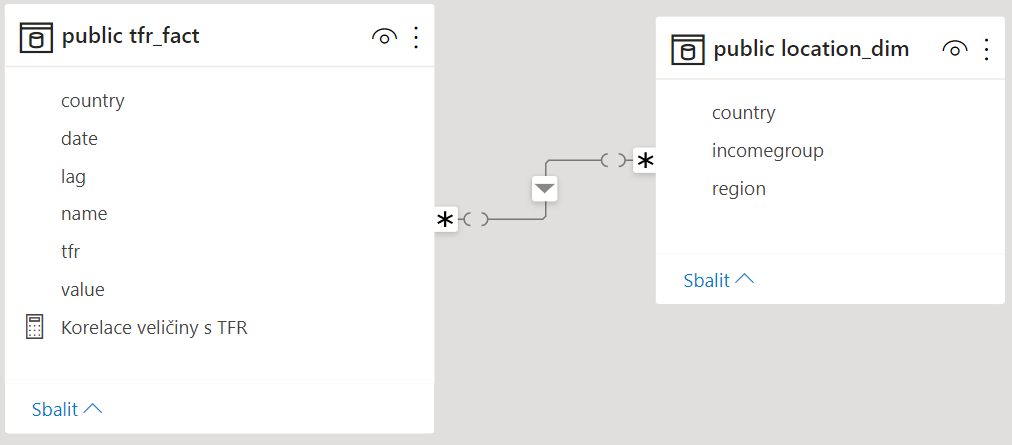
\includegraphics[width=\textwidth]{DP-obrazky/DD_real.png}
    \caption{Obrázek dimenzionální databáze, s kterou pracuje Power BI.}
    \label{fig:DD_Model}
\end{figure}

Zjednodušený reálný model již obsahuje pouze dvě tabulky a veličiny z dimenzionálních tabulek jsou nyní součástí faktové tabulky. Dále zde mám nastavenou novou míru, která počítá korelaci mezi zvolenou veličinou a TFR. Ta slouží pro okamžité zobrazení dané hodnoty, neboť zbylé statistické hodnoty jsou počítány pomocí python skriptu, který je přímo součástí vizuálu, ale zde dochází často k částečnému zpoždění, než jsou dané hodnoty zobrazeny.

\section{Vytvoření datového skladu}

Pro vytvoření kompletního datového skladu se všemi daty na vlastní straně je potřeba mít nainstalovanou PostgreSQL databázi, Pentaho Data Integration, Python 3.0+ s příslušnými knihovnami zmíněnými v kapitole Návrh datového skladu a pro následnou analýzu za pomocí dashboardu Power BI. 

Kompletní návod je součástí souboru Manual v přiložené složce. Všechny datové soubory jsou také již součástí složky a není tedy třeba je stahovat znovu. Po vytvoření všech potřebných komponent a nastavení všech cest a proměnných dle manuálu lze následně celý sklad automaticky vytvořit spuštěním Pentaho Jobu s názvem \textit{Create\_DWH}, jehož struktura je na následujícím obrázku.

\begin{figure}
    \centering
    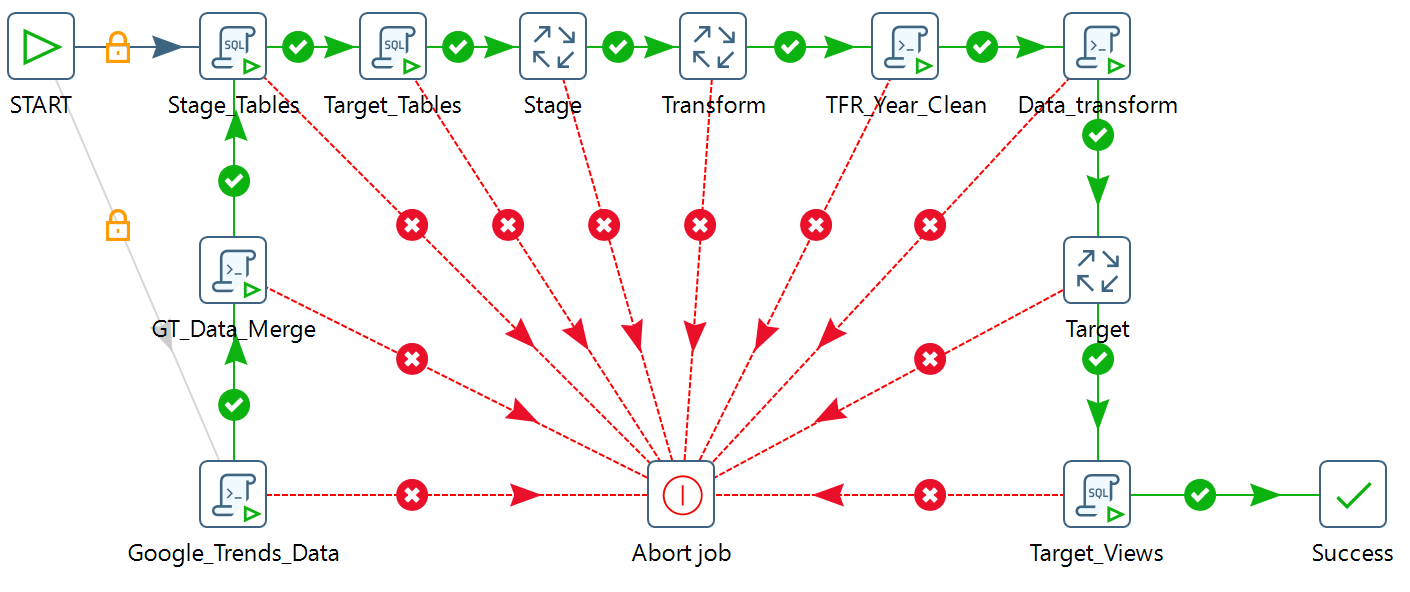
\includegraphics[width=\textwidth]{DP-obrazky/Create_DWH.png}
    \caption{Pentaho Job pro vytvoření datového skladu. Spouští k tomu postupně všechny potřebné skripty a Pentaho Joby.}
    \label{fig:Create_DWH_ETL}
\end{figure}

Součástí Jobu jsou i skripty pro stahování datových sad z Google Trends a jejich následné spojení do jednoho souboru. Tato část je primárně odpojena, neboť při stahování většího objemu dat je toto API chráněno proti přetížení, a proto tento skript obsahuje sleep, který má minimalizovat šanci na nucené ukončení ze strany Googlu. Díky tomu ovšem tento skript může běžet dlouhé hodiny a i přes obsažené čekání může server vyhodit chybu a proces ukončit. Tyto data jsou ovšem již stažena a skript lze využít pro samotné stahování nových datových sad.

Když je kompletně vytvořen celý datový sklad (Create\_DWH job skončil úspěchem), lze následně na přiložený Dashboard připojit vytvořené náhledy a vložit tak do vizuálů aktuální data a začít vlastní analýzu.

Při vkládání vlastních nových datových sad je třeba vytvořit pro tyto sady nové Transakce v Pentaho DI a pro kompletní vytvoření je vhodně zařadit do stromové struktury. Při ukládání nových dat do Target databáze je třeba dodržet danou datovou strukturu a celý soubor vhodně transformovat.

\chapter{Analýza a zobrazení výsledků}

V této kapitole se budu věnovat převážně analýze a interpretaci výsledků, ke kterým jsem pomocí nástrojů BI došel. Budu zde blíže rozebírat jejich vizualizaci a význam jednotlivých prvků zobrazení, aby mohl uživatel sám zkoumat jednotlivé hodnoty, které toto zobrazení nabízí. K tomu, aby byly tyto výsledky poskytnuty co nejširšímu množství uživatelů, je jejich interaktivní dashboard publikován na webové stránky.

V poslední části se budu věnovat vlastní interpretaci výsledků, ve které shrnu celkové výsledky pro vybrané veličiny a zhodnotím možné silné korelanty. Následně se budu věnovat bližší analýze zajímavých veličin, které sice nemusí z celkových výsledků dát silnou korelaci a být tak velký ovlivňovatel TFR, ale existuje u nich nějaký výrazný trend, který je zajímavý a při jeho vhodném aplikování může s dalšími faktory pomoci zvýšit porodnost, ať celkově nebo v určitých zemích, s jejíž kulturou je tento fenomén spojen.


\section{POWER BI}

Jedná se o interaktivní software pro vizualizaci dat, primárně zaměřený na business intelligence. Je vyvíjen společností Microsoft od roku 2011 a je součástí Microsoft Power Platform. Podporuje přímé datové vstupy z databází, souborů (CSV, XML, JSON, spreadsheets,...) nebo webových stránek. 

Tato aplikace existuje jak v Desktopové verzi, tak v Cloudové, kde funguje metodikou Software as a service. Dále obsahuje další komponenty, které slouží k připojení dalších periferií, jako jsou mobilní telefony či jiné služby, díky čemuž má uživatel neustálý přístup ke všem svým vizuálům.

V této aplikaci jsem prováděl hlavní část analýzy faktorů ovlivňujících TFR. Využil jsem jejích bohatých možností pro připojení dat a jejich vzájemné propojení pomocí vizuálního modelu jednotlivých tabulek. Poté jsem využil valstní tvorby dashboardů, které jsem sestavoval z široké palety vizuálních prostředů a filtrů, které tato aplikace nabízí.

\section{Dashboard}

Dashboard je vytvořen, tak aby dával co největší možnost při nastavování různých kritérií, pro něž se následně vypočítávají potřebné statistické ukazatele.

\begin{figure}[h]
    \centering
    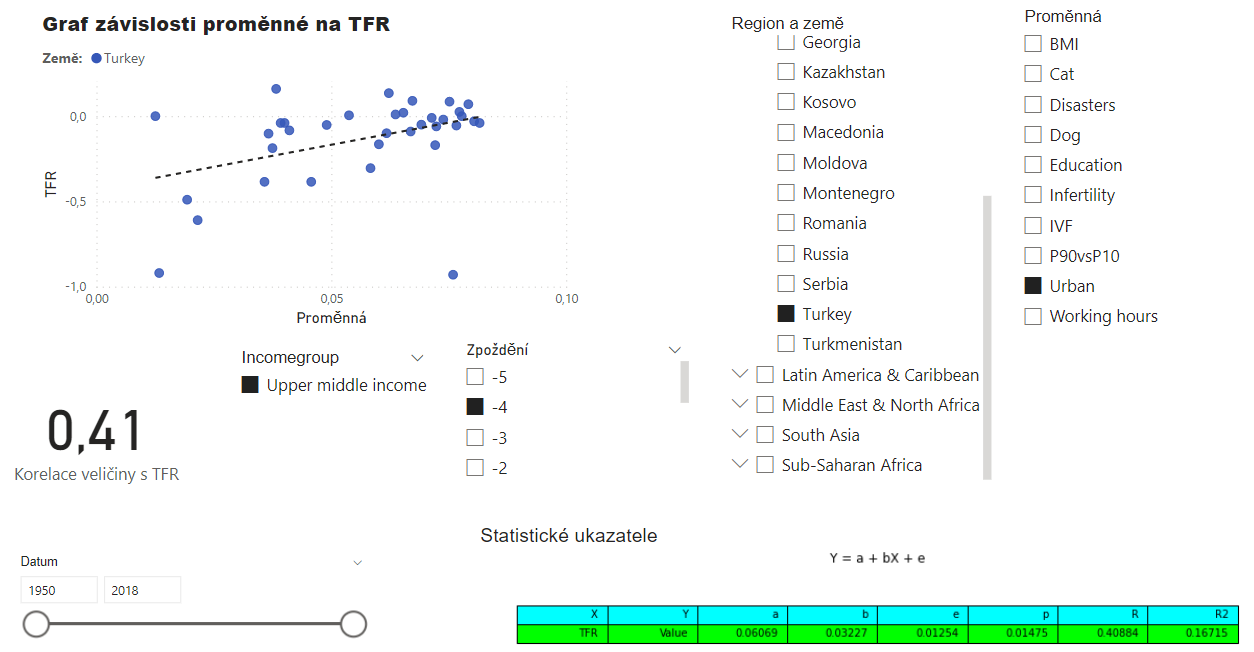
\includegraphics[width=\textwidth]{DP-obrazky/dashboard_mine.png}
    \caption{Ukázka mnou navrženého dashboardu v Power BI.}
    \label{fig:Muj_dashboard}
\end{figure}

Hlavní součástí je samotný graf, který zobrazuje závislost proměnné na TFR, a všechny vybrané státy jsou barevně odlišeny. V grafu je také proložená přímka, která značí vizualizuje lineární regresi pro dané hodnoty.

Dále je tu tabulka se statistickými ukazateli, která zobrazí jak základní parametry pro danou regresní přímku, tak statistické ukazatele, kterými jsou p-hodnota, korelační koeficient \textit{R} a deterministický koeficient $R^2$. Zároveň tato tabulka mění barvu podle toho, jestli je p-hodnota vyšší než 5\% hranice, pak daná tabulka zčervená, a nebo nižší, kdy tabulka změní barvu na zelenou. Protože je pro tuto část vizuálu použit vložený python script, může jeho zobrazení kratší dobu trvat.

Také je zde samotný ukazatel korelace, který již zobrazuje hodnotu bez zpoždění, a je tak možné sledovat pro rychlé hledání pouze tuto hodnotu a nebo ji využít pro kontrolu hodnot v tabulce (když se shoduje s hodnotou \textit{R}, pak je tabulka již aktualizovaná).

Kromě těchto ukazatelů jsou zde všechny potřebné filtry hodnot, jedním z nich je časový, který je nastaven ve formátu od-do, ale lze přepnout i do formátu výběru pro zkoumání vývoje hodnoty v různých zemích v daném roce. Dalším filtr umožňuje vybírat země dle jejich příjmu a tím sjednotit ekonomicky podobně vyspělé skupiny.

Další filtru umožňuje dané testované veličiny vůči sobě časově opožďovat, díky čemuž lze najít nějaký ideální trend v tom, jak rychlý má daná proměnná vliv na TFR či naopak. Asi nejdůležitějším filtrem je samotný výběr proměnné, kterou chceme s hodnotami TFR porovnávat. Jejich názvy koresponduji s názvy u sloupce name v databázi.

Poslední je možnost filtrování regionů a zemí, což kromě přidaného vizuálu umožňuje přímo i graf, kde jsou jednotlivé země umístěny v horní části grafu a při výběru jedné z nich je daná země v grafu zvýrazněná a hodnoty u ukazatelů se přepočítají pro tuto zemi.

\section{Webové stránky}
Osobně si myslím, že jednou z možností, jak TFR zvýšit, je i rozšiřovat povědomí o tomto problému mezi lidmi, aby si uvědomili, že mít děti je důležité. Z tohoto důvodu chci, kromě samotného zkoumání různých korelantů, dát širokému okolí možnost si sami tyto vazby a vztahy prohlédnout. Toho mám v plánu docílit založením webových stránek, které budou obsahovat můj interaktivní dashboard, a dá jim tak možnost nahlédnout do vizualizací a prostých statistických čísel, které dávají různé veličiny ve vztahu k TRF.

Samotný dashboard je hlavním obsahem těchto stránek, a tak se zde budu věnovat převážně jemu a jak je možné publikovat tyto interaktivní analytické vizuály na stránky přímo z Power BI. Celý svůj dashboard jsem vytvořil v Power BI Desktop, ale ten tuto možnost nemá, je třeba ho nejdříve publikovat do svého online pracovního prostoru, který je součástí balíku Microsoft Office 365. Tato verze má sice, co se vizualizačních a analytických možností týče, trochu menší paletu, ale je tu možnost sdílet tento pracovní dashboard na webové stránky. 

Pro tuto možnost lze vygenerovat kód, který lze vložit do přímo do kódu stránky, a po jejím načtení se načte i samotný dashboard, pokud je sdílený či originální dashboard aktivní. Pro plynulost práce s dashboardem a zajištění dostupnosti i při větší vytíženosti ze strany koncových uživatelů se dashboard na klientské strane cachuje. Z tohoto důvodu se všechny změny v originální verzi okamžitě nepropisují a je třeba je buď propsat nuceným kompletním načtením dané stránky a nebo po uplynutí TTL (Time to live) dané cache, která se následné aktualizuje sama.

Samotný dashboard funguje v tomto zobrazení identicky jako v samotné aplikaci. Uživatel zde může libovolně změnit zobrazované hodnoty pomocí filtrů, které jsou zde pro všechny primární dimenze. Vizuály, které zobrazují buď číselné, nebo grafické výsledky, se tomuto výběru interaktivně přizpůsobují a při najetí myší na určitý bod v grafu lze i zobrazit detail pro danou hodnotu (rok, hodnota, země).

Samotné stránky jsou aktuálně vytvořeny na mém Google účtu a od kaz na ně je zde: 

\url{https://sites.google.com/view/totalfertilityrate/domovsk%C3%A1-str%C3%A1nka}

V jejich stránky jsem se snažil držet minimalismu, a proto je zde ustředním faktorem právě daný dashboard a krom toho jen úvodní odstavec, který spojuje dané stránky s touto prací a následně pár vět, které návštěvníkům přiblíží problematiku TFR.

\section{Interpretace výsledků}
V této kapitole bych rád shrnul výsledky pro všechny veličiny, které jsem vůči TFR porovnával a u kterých jsem se domníval, že by mohly mít na tuto veličiny nějaký významný vliv, ať už kladný, nebo záporný. Od předchozích kapitol a hlavně od samotného dashboardu se toto shrnutí liší v tom, že obsahuje komplexní výsledky pro všechny hodnoty, a ukazuje tak, jak si dané veličiny v porovnání s TRF vedou napříč všemi roky a zeměmi, pro které byla data vyhodnocována. Na druhou stranu dashboard dává, více než tento ucelený pohled, možnost uživateli zkoumat dané vztahy více do hloubky, díky všem možným filtrům, díky kterým lze nastavovat parametry všemi možnými směry z pohledu dimenzionální databáze.

Pro výpočet této statistiky jsem opět vytvořil krátký program v pythonu (stat\_sum.py), který vezme data, jež jsou uložena v databázi v podobě pohledu tfr\_fact, a  který tyto data pro každou veličinu zvlášť statisticky porovnájí s veličinou TFR. Tento výpočet se provádí za pomocí knihovny scipy, jež testuje lineární regresi mezi danými hodnotami pro každou zemi. Ty země, kde se s pravděpodobností na 95 procent potvrdí, že tyto veličiny korelují, se přičtou do počtu statisticky potvrzených (p <= 0.05), a tím se získá celkový počet zemí, kde je tato veličina statisticky významná. Dále se toto provádí pro časové zpoždění veličiny o -5 až 5 let a vybere se taková hodnota zpoždění, která má nejlepší statistické hodnoty (je významná pro největší počet zemí). Díky této veličině pak lze i vysledovat, kdy lze očekávat nejvýznamnější reakci druhé veličiny při určité výrazné změně té první.  

Výsledky, které jsem tímto výpočtem získal, jsou sumarizovány v tabulce 6.1. Pro každou testovanou veličinu jsou v ní obsaženy tyto hodnoty popořadě:
\begin{itemize}
    \item Celkový počet zemí, pro které se daná veličina testovala.

    
    \item Celkový počet zemí, pro které je lineární regrese potvrzena na hladině pravděpodobnosti 95\%.

    \item Počet zemí, pro něž je korelace kladná (pro ověření, jestli daná veličina ovlivňuje TFR pozitivně, nebo negativně).
    
    \item Nejnižší nalezená hodnota korelačního koeficientu pro danou veličinu, pro níž vyšla lineární regrese statisticky významná.

    \item Nejvyšší nalezená hodnota korelačního koeficientu pro danou veličinu, pro níž vyšla lineární regrese statisticky významná.

    \item Pro jaké zpoždění vyšly nejlepší statistické výsledky.


\end{itemize}
% Please add the following required packages to your document preamble:
% \usepackage{booktabs}
% \usepackage{graphicx}
\begin{table}[h]
\caption{Tabulka s kompletními výsledky korelace jednotlivých veličin vůči TFR}
\resizebox{\textwidth}{!}{%
\begin{tabular}{@{}ccccccc@{}}
\toprule
\textbf{Název veličiny} &
  \textbf{Počet zemí} &
  \textbf{p <= 0.05} &
  \textbf{Kladá korelace} &
  \textbf{Nejnižší korelace} &
  \textbf{Nejvyšší korelace} &
  \textbf{Zpoždění} \\ \midrule
\multicolumn{1}{|c|}{BMI u žen} &
  \multicolumn{1}{c|}{163} &
  \multicolumn{1}{c|}{37} &
  \multicolumn{1}{c|}{19} &
   \multicolumn{1}{c|}{-0.784} &
  \multicolumn{1}{c|}{0.704} &
  \multicolumn{1}{c|}{-4} \\ \midrule
\multicolumn{1}{|c|}{Doba vzdělání} &
  \multicolumn{1}{c|}{141} &
  \multicolumn{1}{c|}{29} &
  \multicolumn{1}{c|}{3} &
  \multicolumn{1}{c|}{-0.679} &
  \multicolumn{1}{c|}{0.49} &
  \multicolumn{1}{c|}{-3} \\ \midrule
\multicolumn{1}{|c|}{Urbanizace} &
  \multicolumn{1}{c|}{172} &
  \multicolumn{1}{c|}{26} &
  \multicolumn{1}{c|}{11} &
  \multicolumn{1}{c|}{-0.76} &
  \multicolumn{1}{c|}{0.56} &
  \multicolumn{1}{c|}{5} \\ \midrule
\multicolumn{1}{|c|}{Kočky} &
  \multicolumn{1}{c|}{113} &
  \multicolumn{1}{c|}{16} &
  \multicolumn{1}{c|}{4} &
  \multicolumn{1}{c|}{-0.79} &
  \multicolumn{1}{c|}{0.537} &
  \multicolumn{1}{c|}{-3} \\ \midrule
\multicolumn{1}{|c|}{Ženská zaměstnanost} &
  \multicolumn{1}{c|}{175} &
  \multicolumn{1}{c|}{14} &
  \multicolumn{1}{c|}{7} &
  \multicolumn{1}{c|}{-0.525} &
  \multicolumn{1}{c|}{0.577} &
  \multicolumn{1}{c|}{-1} \\ \midrule
\multicolumn{1}{|c|}{Katastrofy} &
  \multicolumn{1}{c|}{146} &
  \multicolumn{1}{c|}{11} &
  \multicolumn{1}{c|}{5} &
  \multicolumn{1}{c|}{-0.65} &
  \multicolumn{1}{c|}{0.646} &
  \multicolumn{1}{c|}{1} \\ \midrule
\multicolumn{1}{|c|}{Psi} &
  \multicolumn{1}{c|}{70} &
  \multicolumn{1}{c|}{10} &
  \multicolumn{1}{c|}{3} &
  \multicolumn{1}{c|}{-0.77} &
  \multicolumn{1}{c|}{0.603} &
  \multicolumn{1}{c|}{-4} \\ \midrule
\multicolumn{1}{|c|}{Neplodnost} &
  \multicolumn{1}{c|}{67} &
  \multicolumn{1}{c|}{9} &
  \multicolumn{1}{c|}{4} &
  \multicolumn{1}{c|}{-0.684} &
  \multicolumn{1}{c|}{0.63} &
  \multicolumn{1}{c|}{-4} \\ \midrule
 \multicolumn{1}{|c|}{Pracovní doba} &
  \multicolumn{1}{c|}{65} &
  \multicolumn{1}{c|}{8} &
  \multicolumn{1}{c|}{3} &
  \multicolumn{1}{c|}{-0.484} &
  \multicolumn{1}{c|}{0.368} &
  \multicolumn{1}{c|}{-1} \\ \midrule
\multicolumn{1}{|c|}{Umělé oplodnění} &
  \multicolumn{1}{c|}{72} &
  \multicolumn{1}{c|}{8} &
  \multicolumn{1}{c|}{4} &
  \multicolumn{1}{c|}{-0.59} &
  \multicolumn{1}{c|}{0.764} &
  \multicolumn{1}{c|}{-5} \\ \midrule
\multicolumn{1}{|c|}{P90vsP10} &
  \multicolumn{1}{c|}{26} &
  \multicolumn{1}{c|}{5} &
  \multicolumn{1}{c|}{3} &
  \multicolumn{1}{c|}{-0.47} &
  \multicolumn{1}{c|}{0.545} &
  \multicolumn{1}{c|}{-4} \\ \midrule
\bottomrule
\end{tabular}%
}
\end{table}

Nejlepší výsledky vyšly pro veličinu BMI u žen, která má kromě největšího množství statisticky významných výsledků také velmi vysoké maximum a minimum korelačního koeficientu. Další zajímavé pozorování o této veličině následně shrnuji v samostatné kapitole.

Další významné výsledky vychází pro veličinu Průměrné doby vzdělání, která je již mnoha výzkumy potvrzena jako významný ovlivňovatel hodnoty TFR, a tak je díky tomu zde prokázáno, že moje postupy dávají pro tuto hodnotu očekávané výsledky. Přesto chci tuto veličinu blíže shrnout v samostatné kapitole, neboť se domnívám, že z bližšího zkoumání lze vytěžit zajímavé poznatky.

V samostatné kapitole chci také shrnout třetí nejvýznamnější korelant, kterým je urbanizace, a také trochu blíže rozvést zjištěné výsledky pro domácí mazlíčky (psi a kočky), neboť i u nich dávalo bližší zkoumání poměrně zajímavé výsledky.

Ostatní veličiny již samy o sobě nedávají tak silné výsledky, ovšem důvodů může být více. Například ženská zaměstnanost, která byla velice dobře zkoumána v práci \textit{Influence of women’s workforce participation and pensions on total fertility rate: a theoretical and econometric study} \cite{Evan}, je velmi ovlivněna časovým obdobím, kdy je její vztah zkoumán, a proto v tomto celkovém pohledu nemá tak silně vypovídající váhu. stejně tak to může platit i pro další hodnoty a je třeba pak pro lepší pochopení použit například mnou vytvořený dashboard, ve kterém lze libovolně volit sledované období a i z grafu lze snadno vyčíst, které hodnoty v kterém roce se značně odchylují od zbytku.

V poslední řadě, než se dostaneme k zajímavému shrnutí významných hodnot, lze ještě podotknout, že dalším důležitým faktorem je také to, že nikdy tyto veličiny nepůsobí na TFR jen samy o sobě, a tedy v kombinaci s dalšími hodnotami mohou dávat lepší ucelený výsledek a dostat tak i významnější výsledky. Příkladem by mohla být například kombinace neplodnosti a umělého oplodnění, která v kombinaci s vyhledáváním mohou mít významnou souvislost.


\subsection{BMI}
Jak již bylo řečeno, BMI má, co se týče lineární regrese ve vztahu s TFR, velice dobré výsledky, ale je tu pár věcí, které z těchto strohých výsledků zcela nevyplývají. Asi většina z nás ví, že BMI je tabulkový ukazatel “zdraví”, lépe řečeno poměr váhy ku výšce. Já osobně těmto hodnotám příliš velký význam nepřikládám, protože mnohem důležitější je složení této váhy. Můžeme to demonstrovat na příkladu dvou osob, kdy jedna má BMI optimální, ale přesto trpí takzvanou skrytou obezitou, protože má minimum svalové hmoty a velké množství tuků, zatímco druhá osoba může mít dle BMI nadváhu, ale přitom má klidně méně než 10 \% tělesného tuku a jedná se o silového sportovce s velkým množstvím svalové hmoty.

Ale abych se dostal k tomu hlavnímu, ačkoli BMI není optimální ukazatel, pro průměrný vzorek populace poslouží poměrně rozumně. A s tím souvisí právě vztah k TFR, jak je vidět při porovnání surových hodnot BMI a TFR, nejlepší výsledky pro porodnost jsou právě v ideálních hodnotách BMI. I proto, jak je v tabulce 6.1 vidět, je počet kladných a zapornách korelací vyrovnaná, neboť v některých státech se hodnota BMI pohybuje od nízké k normální, a má tedy korelaci kladnou, a v jiných naopak od normální k vysoké, a pak se to láme a korelace padá k záporným hodnotám. 

Má to hned několik důležitých důvodů. Jedním velmi známým je, že jakýkoliv extrém (velmi nízká hladina tuku i vysoká obezita) vede k přerušení ženských reprodukčních schopností a neplodnosti, i když ne trvalé. Dále s tím souvisí i fyzická přitažlivost a samotná psychická pohoda. Myslím si, že je určitě mnoho dalších faktorů, které se v tomto mohou promítnout, a proto beru tento výsledek za velmi zásadní. 

\begin{figure}
    \centering
    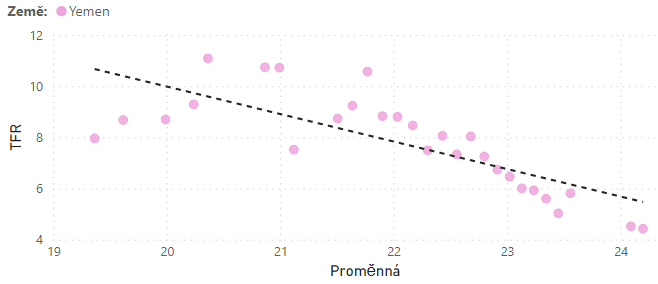
\includegraphics[width=\textwidth]{DP-obrazky/BMI.png}
    \caption{Příklad datové sady, kde je vidět maximum hodnot mezi hodnotami BMI 18 a 25. Když se blížíme k těmto mezním hodnotám, tak hodnoty TFR významně klesají. Jemen byl vybrán, neboť obsahuje obě mezní hodnoty. Jiné země se většinou pohybují pouze v horní nebo dolní části křivky.}
    \label{fig:BMI_Yemen}
\end{figure}

\subsection{Vzdělání}
Jak již bylo popsáno, vzdělání je klíčový faktor, který TFR ovlivňuje, hlavně z důvodu odkladu prvního dítěte na konec studia a ztráty tak drahocenných let, kdy je žena nejplodnější, ale také proto, že vyšší studium otevírá lepší možnosti, jak se pracovně uplatnit a budovat slibnou kariéru. 

Z těchto důvodů, a jak je i z výsledků v tabulce 6.1 zřejmé, je právě doba vzdělání v korelaci s TFR záporná, a tak velmi silně ovlivňuje její pokles. Ovšem co je v tomto případě důležité, je to, že tam funguje určitý vývoj, který přesně kopíruje vliv vývoje od zemí třetího světa až po země vyspělé. Kdy z počátků kdy začne doba vzdělání růst, tak TFR vede k rychlému pádu, ale s postupem času začne brzdit a s každým dalším rokem k době studia je již daný vliv menší a menší. 

Jak jsem již zmínil myslím si, že tento faktor velmi silně souvisí s celkovým přerodem v dané zemi a že odpírat ženám vzdělání určitě není správné řešení. Spíše by mohlo pomoci jim již během studia tuto problematiku osvětlit, aby věděly, jak je důležité mít děti.

\subsection{Urbanizace}
Stejně jako vzdělání, tak i tento faktor silně souvisí s postupným přerodem zemí. I tato veličina má velmi dobré výsledky, a je tedy významným korelantem, ale na druhou stranu je z výsledků vidět, že významná část korelantů nabírá kladnou hodnotu. A také to, že na rozdíl od ostatních je doba zpoždění kladná, což znamená, že TFR reaguje se značným zpožděním na rostoucí míru urbanizace. 

Tyto dvě zásadní věci souvisí hodně na typu urbanizace, která v dané zemi probíhá, protože pokud je to rychlá a neřízená urbanizace, je výsledek korelace většinou záporný a výsledek není nijak silně ovlivněn zpožděním. Hlavním důvodem je právě to, že tato urbanice není řízená, a není tak v daných městech dostatečně rozvinuté zázemí pro děti a lidé jsou mnohem více nuceni pracovat, aby se v městě, které je dražší než venkov, uživili. 

Na druhou stranu je právě pozvolnější přerod, kdy jsou již města na nárůst obyvatel připravena, mají dostatek školek, škol a dalších institucí, kde je o děti postaráno, a tak když se lidé do města nastěhují a po počáteční době, než se zabydlí, stabilizují své příjmy (což je daný lag), se rozhodnou  děti mít, tak je výsledná korelace pozitivní, a jsou to ty hodnoty, které jsou ke statistickým výsledkům přidány až díky zpoždění, neboť bez něj tyto hodnoty nebyly statisticky průkazné.

Toto zjištění může být návodné pro to ukázat, jak kvalitní infrastruktura, která na děti myslí, může podpořit jejich potenciální růst, a pokud se k tomu přidá i zajímavá finanční podpora, která umožní matce být s dítětem na mateřské první roky jeho života, které jsou klíčové pro jeho rozvoj, může to mít pozitivní vliv. 


\subsection{Psi a kočky}
Poslední skupinou, které bych se chtěl blíže věnovat, jsou domácí mazlíčci, lépe řečeno psi a kočky. U této skupiny jsem se domníval, že budou mít spíše negativní efekt,neboť je spousta lidí, kteří si právě těmito mazlíčky děti vynahrazují, a to pak na samotnou porodnost dopadá.

Ovšem problém této skupiny je mnohem složitější, jak jsem při jejím bližším zkoumáním zjistil, a dost se liší stát od státu. Hlavní příčinou může být kulturní odlišnost a to, jak dané země tato zvířata vnímají, ale hlavně i samotný vztah lidí k daným zvířatům a představě rodiny všeobecně. Pomineme-li ovšem ty země, kde nejsou tato zvířata brána jako domácí mazlíčci, a tedy nemá smysl jejich vliv na korelaci v těchto zemích zkoumat, tak se zdá, že se lidé dělí na dva tábory. 

První skupina přesně zapadá do mého předpokladu a zde je vliv dle očekávání negativní a i z výsledků se zdá, že průměrně mazlíčci počet dětí snižují, ale pak je druhá skupina lidí, kteří naopak preferují klasickou představu rodiny, kde k dětem patří právě i domácí mazlíček, jenž je plnohodnotným členem domácnosti. 

Díky této rozpolcenosti jsou pak krásně vidět rozdíly, kdy  například v USA má pes poměrně vysokou negativní korelaci, ale naopak v Německu je silná pozitivní korelace. A díky tomu je i spousta zemí, kde jsou oba tábory dohromady, a díky tomu jsou následně výsledky statisticky neprůkazné a z hodnocení vypadají stejně jako země, kde tato zvířata jako mazlíčky neřeší. Proto je zrovna v tomto případě myslet na tyto další faktory, ale samo o sobě asi nelze brát domácí zvířata jako značné hybatele TFR a jako něco, díky čemu by se mohla její hodnota zvýšit.

\begin{figure}
    \centering
    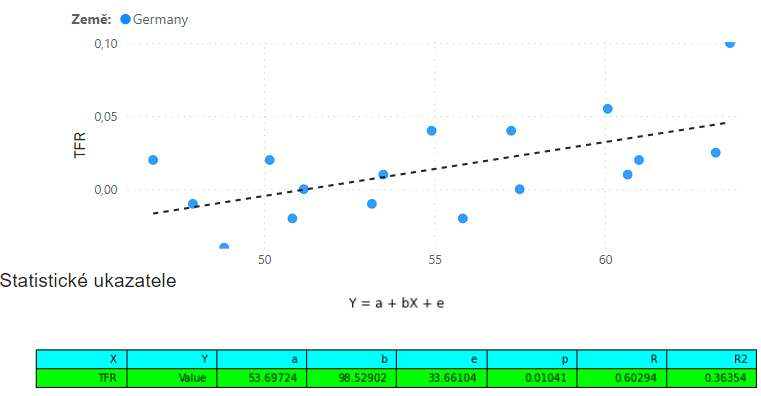
\includegraphics[width=\textwidth]{DP-obrazky/Dog_germany.png}
    \caption{Ukázka vlivu psů na TFR v Německu, kde má významný pozitivní efekt na TFR.}
    \label{fig:Dog_Germany}
\end{figure}
\begin{figure}
    \centering
    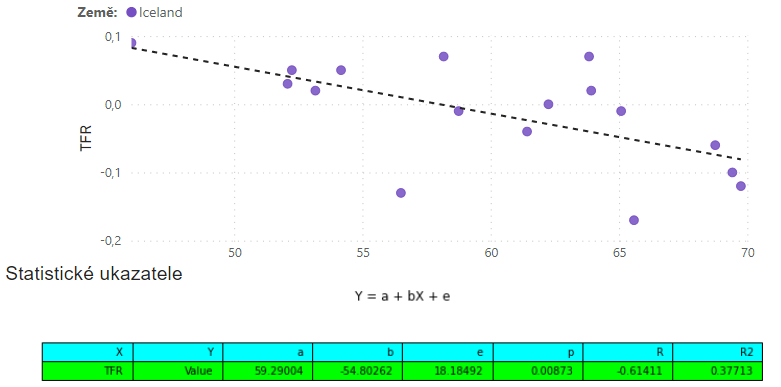
\includegraphics[width=\textwidth]{DP-obrazky/Dog_island.png}
    \caption{Ukázka vlivu psů na TFR na Islandu, kde má významný negativní efekt na TFR.}
    \label{fig:Dog_Island}
\end{figure}


\begin{conclusion}
	V této práci jsem se zabýval analýzou vztahu mezi TFR a mnou vybranými veličinami za pomocí metodiky BI. Z tohoto hlediska bylo nejprve potřeba čtenáři osvětlit používané pojmy a celkovou problematiku TFR. Dále také matematické metody, které byly využity při statistickém vyhodnocování a v poslední řadě byla čtenáři představena metodika BI a veškeré náležitosti, jež s ní souvisí a byly využity pro tvorbu této práce.
	
V praktické části byl navržen a vytvořen datový sklad, ktarý za pomoci automatických skriptů a ETL procesů zpracovává zvolené datové sady do požadovaného formátu (dimenzionální databáze). Z této databáze jsem následně v nástroji Power BI vytvořil interaktivní dashboard, v kterém je možné za pomocí přednastavených filtrů libovolně zkoumat vztahy zvolených veličin. Tento nástroj jsem následně publikoval na webové stránky, které jsem za tímto účelem vytvořil, abych tím umožnil přístup co nejvíce uživatelům a mohl tak šířit větší povědomí o této problematice.

Na závěr jsem dané veličiny sám statisticky vyhodnotil a zároveň jsem uvedl zajímavé poznatky, které z bližší analýzy ve vytvořeném dashboardu vyplynuly.

Součástí práce jsou také veškeré zdrojové kódy a manuál, který je určen pro uživatele, kteří by si rádi tento datový sklad postavili u sebe na stanici. Také je zde návod, jak přidat další datové sady, které dané uživatelé zajímají, a zkoumat tak nové možnosti.

\end{conclusion}

%\bibliographystyle{csn690}
%\bibliography{mybibliographyfile}
\begin{thebibliography}{99}
\bibitem{openknowlidge}\textit{Determinants and Consequences of High Fertility: A Synopsis of the Evidence}, [online], 2010, [cit. 2022-09-17], Dostupné z: \url{https://openknowledge.worldbank.org/bitstream/handle/10986/27497/630690WP0P10870nants0pub08023010web.pdf?fbclid=IwAR2mLj5BF1I13tUA7SrMKAQOJKwKBCwU7toPE5j6fkoktahHV5nmraGeNfA}

\bibitem{UN-TFR}\textit{United Nations, Population Division, United Nations publication, Sales No. E.06.XIII.5, New York, 2006}, [cit. 2022-09-17], Dostupné z: \url{https://www.un.org/esa/sustdev/natlinfo/indicators/methodology_sheets/demographics/total_fertility_rate.pdf}

\bibitem{Götmark}\textit{Götmark, F., Andersson, M. Human fertility in relation to education, economy, religion, contraception, and family planning programs.} BMC Public Health 20, 265, 2020. \url{https://doi.org/10.1186/s12889-020-8331-7}

\bibitem{CHOI}\textit{CHOI, Yoonjoung, Madeleine SHORT FABIC a Jacob ADETUNJI. Does age-adjusted measurement of contraceptive use better explain the relationship between fertility and contraception?}. Demographic Research [online]. 2018, 39, 1227-1240 [cit. 2022-09-25]. ISSN 1435-9871. Dostupné z: \url{doi:10.4054/DemRes.2018.39.45}

\bibitem{Girum}Girum \textit{T, Wasie A. Return of fertility after discontinuation of contraception: a systematic review and meta-analysis.} Contracept Reprod Med. 2018 Jul 23,3:9. [cit. 2022-09-21], doi: 10.1186/s40834-018-0064-y. PMID: 3006204, PMCID: PMC6055351.

\bibitem{Yujie} \textit{Yujie, Li, The Relationship between Fertility Rate and
Economic Growth in Developing Countries}, Supervisor: Martin Dribe, [Master thesis], 2015, [cit. 2022-09-25], Dostupné z: \url{https://lup.lub.lu.se/luur/download?func=downloadFile&recordOId=8727479&fileOId=8768892&fbclid=IwAR1e53pDkNj2nRrq_tmOOiIDv2IQp2q33yziVQD4iaIsJWPNV0ADcNfklo}

\bibitem{Pourreza} \textit{Pourreza, A., Sadeghi, A., Amini-Rarani, M. et al. Contributing factors to the total fertility rate declining trend in the Middle East and North Africa: a systemic review.} J Health Popul Nutr 40, 11 (2021).[cit. 2022-09-25], \url{https://doi.org/10.1186/s41043-021-00239-w}

\bibitem{Evan} \textit{EVAN, Tomáš a Pavla VOZÁROVÁ. Influence of women’s workforce participation and pensions on total fertility rate: a theoretical and econometric study.} Eurasian Economic Review [online]. 2018, 8(1), 51-72 [cit. 2022-09-25]. ISSN 1309-422X. Dostupné z: doi:10.1007/s40822-017-0074-0

\bibitem{Martine} \textit{Martine, George, Jose Eustaquio Alves, and Suzana Cavenaghi. Urbanization and Fertility Decline: Cashing in on Structural Change.} International Institute for Environment and Development, 2013. [cit. 2022-09-24], \url{http://www.jstor.org/stable/resrep01293}.

\bibitem{brotz} \textit{BROTZ, Daniel. Hledání a práce s veličinami souvisejícími s TFR.} Praha, 2022. Bakalářská práce. ČVUT Fakulta informačních technologií. Vedoucí práce Evan Tomáš.

\bibitem{Kuznets} \textit{Kuznets, Simon. “Rural-Urban Differences in Fertility: An International Comparison.”} Proceedings of the American Philosophical Society, vol. 118, no. 1, 1974, pp. 1–29. JSTOR, [cit. 2022-09-25], \url{http://www.jstor.org/stable/986434}. 

\bibitem{UN-PD}\textit{United Nations, Population Division, FERTILITY LEVELS AND TRENDS IN COUNTRIES WITH INTERMEDIATE LEVELS OF FERTILITY}, 2002, [cit. 2022-09-17], Dostupné z: \url{https://www.un.org/development/desa/pd/sites/www.un.org.development.desa.pd/files/unpd_egm_200203_backgroundpaper_fertility_levels_and_trends_population_division.pdf?fbclid=IwAR1KiGoqZgvyzqFxhuB_QcIbZVPZQ9uGmMNHcMCDDESWKzksB9krimSA5Ew}

\bibitem{krivy} \textit{KŘIVÝ, Ivan. ANALÝZA ČASOVÝCH ŘAD} [online]. Ostrava, 2012 [cit. 2022-09-29]. Dostupné z: \url{https://web.osu.cz/~Bujok/files/ancas.pdf.} Skripta. Ostravská univerzita v Ostravě.

\bibitem{blazek} \textit{BLAŽEK, B., Jitka HRABÁKOVÁ, Pavel HRABÁK, Roman KOTECKÝ, Petr NOVÁK a Daniel VAŠATA. Testování hypotéz: 10. přednáška} [online]. Praha, 2011 [cit. 2022-09-29]. Dostupné z: \url{https://courses.fit.cvut.cz/NI-VSM/lectures/files/NI-VSM-Lec-10-Slides.pdf}. Učební materiál. ČVUT.

\bibitem{korelace} \textit{BLAŽEK, B., Jitka HRABÁKOVÁ, Pavel HRABÁK, Roman KOTECKÝ, Petr NOVÁK a Daniel VAŠATA. Náhodné vektory: 3. přednáška} [online]. Praha, 2011 [cit. 2022-09-29]. Dostupné z: \url{https://courses.fit.cvut.cz/NI-VSM/lectures/files/NI-VSM-Lec-03-Slides.pdf}. Učební materiál. ČVUT.

\bibitem{linreg} \textit{Jednoduchá lineární regrese} [online]. Brno, 2022 [cit. 2022-09-29]. Dostupné z: \url{https://mathstat.econ.muni.cz/media/19031/linearni-regrese.pdf}. Učební materiál. Masarykova univerzita.

\bibitem{AJCR} \textit{Základy ekonometrie: IX. Analýza jednorozměrných časových řad} [online]. Brno, 2015 [cit. 2022-09-29]. Dostupné z: \url{https://is.muni.cz/el/1456/podzim2015/BKE_ZAEK/um/59125597/09_CasRady.pdf}. Učební materiál. Masarykova univerzita.

\bibitem{pokorny} \textit{POKORNÝ, Martin. Testy jednotkového kořene a jejich využití v ekonomii} [online]. Brno, 2012 [cit. 2022-09-29]. Dostupné z: \url{https://is.muni.cz/th/uzm4g/DIPLOMOVA_PRACE.pdf}. Diplomová práce. Masarykova univerzita. Vedoucí práce Ing. Daniel Němec, Ph.D.

\bibitem{EDW1} \textit{KOLÁŘ, Robert a Jakub KREJČÍ. Podnikové datové sklady: 1. přednáška} [online]. Praha, 2022 [cit. 2022-09-29]. Dostupné z: \url{https://courses.fit.cvut.cz/NI-EDW/lectures/01_prednaska.pdf}. Učební materiál. ČVUT.

\bibitem{EDW2} \textit{KOLÁŘ, Robert a Jakub KREJČÍ. Podnikové datové sklady: 2. přednáška} [online]. Praha, 2022 [cit. 2022-09-29]. Dostupné z: \url{https://courses.fit.cvut.cz/NI-EDW/lectures/02_prednaska.pdf}. Učební materiál. ČVUT.

\bibitem{EDW-C1} \textit{KOLÁŘ, Robert a Jakub KREJČÍ. Podnikové datové sklady: 1. cvičení} [online]. Praha, 2022 [cit. 2022-09-29]. Dostupné z: \url{https://courses.fit.cvut.cz/NI-EDW/tutorials/01_cviceni.pdf}. Učební materiál. ČVUT.

\bibitem{EDW3} \textit{KOLÁŘ, Robert a Jakub KREJČÍ. Podnikové datové sklady: 3. přednáška} [online]. Praha, 2022 [cit. 2022-09-29]. Dostupné z: \url{https://courses.fit.cvut.cz/NI-EDW/lectures/03_prednaska.pdf}. Učební materiál. ČVUT.

\bibitem{EDW4} \textit{KOLÁŘ, Robert a Jakub KREJČÍ. Podnikové datové sklady: 4. přednáška} [online]. Praha, 2022 [cit. 2022-09-29]. Dostupné z: \url{https://courses.fit.cvut.cz/NI-EDW/lectures/04_prednaska.pdf}. Učební materiál. ČVUT.

\bibitem{EDW5} \textit{KOLÁŘ, Robert a Jakub KREJČÍ. Podnikové datové sklady: 5. přednáška} [online]. Praha, 2022 [cit. 2022-09-29]. Dostupné z: \url{https://courses.fit.cvut.cz/NI-EDW/lectures/05_prednaska.pdf}. Učební materiál. ČVUT.

\bibitem{kapustova} \textit{KAPUSTOVÁ, Veronika. Cvičební pomůcka pro předmět Základy statistiky pro přírodní vědy}. Ostrava 2021, [cit. 2022-09-29], Učební materiál. Ostravská univerzita v Ostravě.

\bibitem{python} \textit{Download Python | Python.org. Welcome to Python.org} [online]. Copyright ©2001 [cit. 23.8.2022]. Dostupné z: \url{https://www.python.org/downloads/}

\bibitem{postgres} \textit{PostgreSQL: Downloads. PostgreSQL: The world's most advanced open source database} [online]. Copyright © 1996 [cit. 23.8.2022]. Dostupné z: \url{https://www.postgresql.org/download/}

\bibitem{postbird} \textit{Postbird | Apps | Electron. Electron | Build cross-platform desktop apps with JavaScript, HTML, and CSS.} [online]. Dostupné z: \url{https://electron-website.herokuapp.com/apps/postbird}

\bibitem{EA} \textit{Full Lifecycle Modeling for Business, Software and Systems | Sparx Systems.} UML modeling tools for Business, Software, Systems and Architecture [online]. Copyright © 2000 [cit. 28.8.2022]. Dostupné z: \url{https://sparxsystems.com/products/ea/}

\bibitem{pentaho} \textit{Installing Pentaho Data Integration CE | Hitachi Vantara.} [online]. Copyright © Hitachi Vantara LLC 2022. All Rights Reserved. [cit. 28.8.2022]. Dostupné z: \url{https://www.hitachivantara.com/en-us/pdf/implementation-guide/three-steps-to-install-pentaho-data-integration-ce.pdf}

\bibitem{VSC} \textit{Visual Studio Code - Code Editing. Redefined. Visual Studio Code - Code Editing. Redefined} [online]. Copyright © 2022 Microsoft [cit. 23.8.2022]. Dostupné z: \url{https://code.visualstudio.com/}

\bibitem{powerbi} textit{Vizualizace dat | Microsoft Power BI. Object moved} [online]. Copyright © 2022 Microsoft [cit. 31.8.2022]. Dostupné z: \url{https://powerbi.microsoft.com/cs-cz/}

\bibitem{pytrends} \textit{pytrends · PyPI. PyPI · The Python Package Index} [online]. Copyright © 2022 [cit. 28.8.2022]. Dostupné z: \url{https://pypi.org/project/pytrends/}

\bibitem{CC} \textit{country-converter · PyPI. PyPI · The Python Package Index} [online]. Copyright © 2022 [cit. 28.8.2022]. Dostupné z: \url{https://pypi.org/project/country-converter/}

\bibitem{stat} \textit{Introduction — statsmodels.} [online]. [cit. 28.8.2022]. Dostupné z: \url{https://www.statsmodels.org/stable/index.html}

\bibitem{numpy} \textit{NumPy. NumPy} [online]. Copyright © 2022 NumPy. All rights reserved. [cit. 28.8.2022]. Dostupné z: \url{https://numpy.org/}

\bibitem{pandas} \textit{pandas - Python Data Analysis Library. pandas - Python Data Analysis Library} [online]. Copyright © 2022 pandas via [cit. 28.8.2022]. Dostupné z: \url{https://pandas.pydata.org/}

\bibitem{google} \textit{Google Trends.} [online].[cit. 24.7.2022]. Dostupné z: \url{https://trends.google.com/trends/?geo=CZ}

\bibitem{worldbank} \textit{World Bank Open Data | Data. World Bank Open Data | Data} [online]. Copyright © [cit. 24.7.2022]. Dostupné z: \url{https://data.worldbank.org/}

\bibitem{OWD} \textit{Our World in Data. Our World in Data} [online]. [cit. 28.7.2022]. Dostupné z: \url{https://ourworldindata.org/}

\bibitem{BMI} \textit{Mean body mass index (BMI) in women - Our World in Data. Our World in Data} [online]. [cit. 29.7.2022]. Dostupné z: \url{https://ourworldindata.org/grapher/mean-body-mass-index-bmi-in-adult-women}

\bibitem{p90} \textit{P90 vs. P10 of income/consumption distribution - Our World in Data. Our World in Data} [online]. [cit. 29.7.2022]. Dostupné z: \url{https://ourworldindata.org/grapher/p90-vs-p10-logs}

\bibitem{schooling} \textit{Average years of schooling for women - Our World in Data. Our World in Data} [online]. [cit. 29.7.2022]. Dostupné z: \url{https://ourworldindata.org/grapher/mean-years-of-schooling-female}

\bibitem{urban} \textit{Number of people living in urban and rural areas - Our World in Data. Our World in Data} [online]. [cit. 29.7.2022]. Dostupné z: \url{https://ourworldindata.org/grapher/urban-and-rural-population}

\bibitem{working hours} \textit{Annual working hours per worker - Our World in Data. Our World in Data} [online]. [cit. 29.7.2022]. Dostupné z: \url{https://ourworldindata.org/grapher/annual-working-hours-per-worker}

\bibitem{disasters} \textit{Death rate from natural disasters - Our World in Data. Our World in Data} [online]. [cit. 29.7.2022]. Dostupné z: \url{https://ourworldindata.org/grapher/death-rates-from-disasters}

\bibitem{country} \textit{Fertility rate, total (births per woman) | Data. World Bank Open Data} | Data [online]. Copyright © [cit. 26.7.2022]. Dostupné z: \url{https://data.worldbank.org/indicator/SP.DYN.TFRT.IN}

\bibitem{labor} \textit{Labor force, female (\% of total labor force) | Data. World Bank Open Data} | Data [online]. Copyright © [cit. 26.7.2022]. Dostupné z: \url{https://data.worldbank.org/indicator/SL.TLF.TOTL.FE.ZS}

\bibitem{fr} \textit{World Fertility Data | Population Division. Welcome to the United Nations} [online]. Dostupné z: \url{https://www.un.org/development/desa/pd/data/world-fertility-data}


\end{thebibliography}

\appendix

\chapter{Seznam použitých zkratek}
% \printglossaries
\begin{description}
    \item[API] Application Programming Interface
    \item[AR] Autoregresivní
	\item[BI] Business intelligence 
	\item[BMI] Body Mass Index
	\item[CSV] Comma-separated values
	\item[DDL] Data Definition Language
	\item[DI] Data integration
	\item[DWH] Data Warehouse
	\item[ETL] Extract, Transform, Load
	\item[IDE] Integrated Development Environment
	\item[iid] Independent and identically distributed 
	\item[IP] Internet protocol
	\item[KPI] Key performance indikator
	\item[KPSS] Kwiatkowski–Phillips–Schmidt–Shin
	\item[LM] Lagrangeův multiplikátor
	\item[OLS] Ordinary least squares
	\item[SQL] Structured Query Language
	\item[TFR] Total fertility rate
	
\end{description}

\chapter{Malual}
Tato příloha má uživateli pomoci správně nastavit své prostředí a navést ho při práci s ETL nástrojem Pentaho Data Integration.

\section{Vytvoření DWH}
Tato část obsahuje podrobný návod pro vytvoření celého datového skladu v takovém stavu, v jakém je zhotoven pro potřeby této práce.
\subsection{Softwarové požadovky}
Aby bylo možné vytvořit celý sklad automaticky pomocí Pentaho Jobu Create\_DWH, je třeba mít na zařízení následující nástroje:

\begin{itemize}
    \item PostgreSQL databáze
    \begin{itemize}
        \item Stage
        \item Target
    \end{itemize}
    \item Python 3.0+ \cite{python}(+knihovny)
    \begin{itemize}
        \item Pandas
        \item country-converter
        \item pytrends
        \item numpy
        \item statsmodels
    \end{itemize}
    \item Pentaho Data Integration 6.0.0.0-353+
    \item Power BI
\end{itemize}

\subsection{Nastavení proměnné prostředí}
V nástroji pro správu ETL procesů je třeba nastavit správně proměnné prostředí, které slouží pro správnou práci se soubory a skripty. Postup je následující:
Zvolte \textbf{Edit -> Set Enviromental Variables}.
Zde je možné nastavit dvě proměnné:

\begin{enumerate}
    \item \textbf{path} - kam vložíte celou cestu k odresáři, kde je vložena kompletní složka DP-data (např. C:\textbackslash Program Files (x86))
    \item \textbf{python} - zde vložíte cestu k python kompilatoru, který má přístup ke všem potřebným knihovnám 
    
    (např. C:\textbackslash Users\textbackslash AppData\textbackslash Local\textbackslash Microsoft\textbackslash WindowsApps\textbackslash python.exe)

\end{enumerate}

\subsection{Připojení databáze}
Pro správnou funkčnost je třeba změnit připojení obou dílčích databází na ty, které máte vytvořeny na vlastním stroji. Postup je následující:
\begin{enumerate}
    \item Otevřete Pentaho Job Create\_DWH
    \item Na boční Tool liště zvolte \textbf{View->Jobs->Create\_DWH->Database connections}
    \item Zde klikněte pravým tlačítkem na jednotlivé FR připojení, zvolte možnost \textbf{edit} a následně v okénku wizzardu nastavte připojení na vlastní databazi Stage či Target
    
\end{enumerate}

\begin{figure}
    \centering
    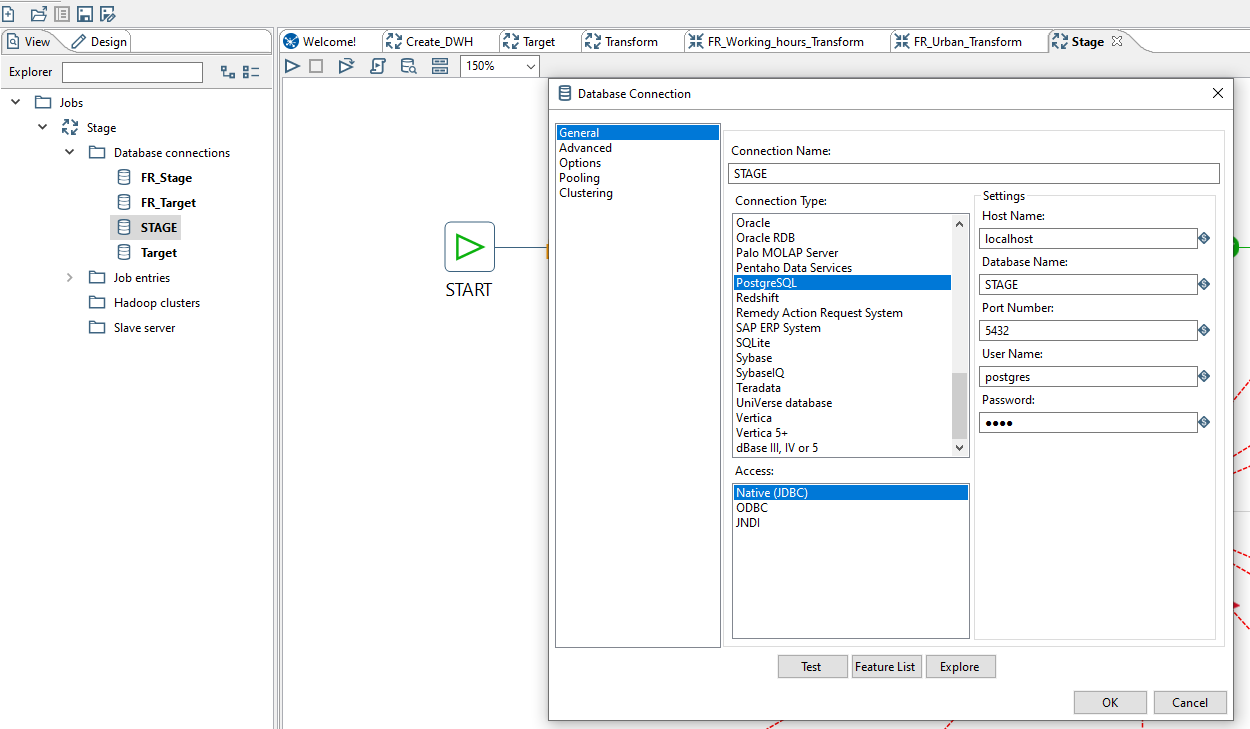
\includegraphics[width=\textwidth]{DP-obrazky/nastaveni_databaze.png}
    \caption{Obrázek k návodu k připojení databází v Pentaho DI.}
    \label{fig:Pentaho_database}
\end{figure}

\subsection{Propojení Power BI s databází}
Po otevření již připraveného FR\_Dashboardu by měly být data součástí sestavy. Pokud chcete data aktualizovat nebo dashboard napojit přímo na vlastní databázi, stačí postupovat dle popisu dále:
\begin{enumerate}
    \item V záložce \textbf{Domů\textbackslash Home -> Získat data\textbackslash Get data -> Více\textbackslash More -> Databáze\textbackslash Database -> databáze PostgreSQL}
    \item Dále vyplňte údaje potřebné pro připojení vlastní databáze a zvolte potřebné tabulky náhledů, ze kterých je vytvořen datamart a z jehož dat se vytváří vlastní vizualizace.
\end{enumerate}

\section{Přidání datové sady do DWH}
Datový soubor by měl mít příponu .csv, a být uložen ve složce:

DP-data\textbackslash Original\_Data\_Sources.

Pentaho DI samozřejmě podporuje i jiné typy datových souborů a lze je tedy bez problému nahrát, ale v tomto případě nelze využít možnosti se v nastavení jednotlivých částí transakce inspirovat již předpřipravenými částmi. 

Do SQL souboru FR\_Stage lze doplnit část pro vytvoření tabulky pro daný soubor a nebo je možné nechat vytvořit tabulku přímo z Pentaho DI, který rovnou i zobrazí kompletní SQL kód, který lze následně do tohoto souboru jen zkopírovat pro případné znovuvytvoření celého skladu.

Zbylé tabulky již nejsou při přidávání souboru ovlivněny, a tak stačí již pouze správně vytvořit ETL transakce a přiřadit je do Správného Jobu. 

\subsection{Vytvoření transakce pro Stage}
Po zvolení možnosti \textbf{Vytvořit novou transakci} je nutné z toolboxu zvolit \textbf{CSV file input}, v něm vybrat vámi stažený soubor. Popřípadě zvolit jinou možnost inputu dat, dle vaší situace.
Po vložení správného souboru a zvolení správného nastavení dle vlastností dat a souboru, lze vybrat \textbf{Get Fields}. Nahrají se všechny sloupce dle hlaviček CSV souboru. Následně je třeba upravit datové typy  a nejspíš bude třeba u určitých hodnot zvolit vyšší hodnotu \textbf{Length}, aby všechny data bez problému prošla, protože přednastavené velikosti jsou určeny pouze z menšího vzorku a ne celého souboru, a tak nemusí odpovídat realitě.

\begin{figure}
    \centering
    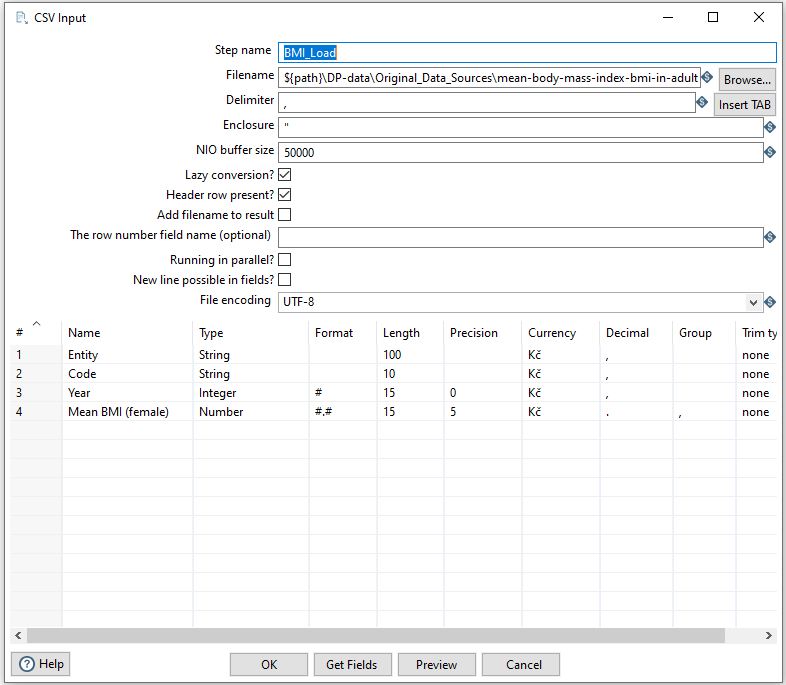
\includegraphics[width=\textwidth]{DP-obrazky/CSV_input.png}
    \caption{Ukázka nastavení hodnot pro CSV input.}
    \label{fig:CSV_input}
\end{figure}

Následně zvolte z Toolbaru \textbf{Table output} a spojte s předchozím krokem ve správném směru šipky. Připojte k ní \textbf{Stage} databázi s tabulkou pro tyto data. Zvolte \textbf{Truncate table} a \textbf{Specify database fields}. Následně klikněte na \textbf{Database fields}, kde zvolíte \textbf{Get fields}. 

Pokud nemáte již připravenou tabulku, stačí zvolit možnost \textbf{SQL} a vygeneruje se kód pro její vytvoření a zároveň je tabulka s vámi zvoleným názvem (ten by neměl kolidovat s již vzniklými tabulkami, jinak budou přepsány) vytvořena na databázovém stroji \textbf{Stage}.

\begin{figure}
    \centering
    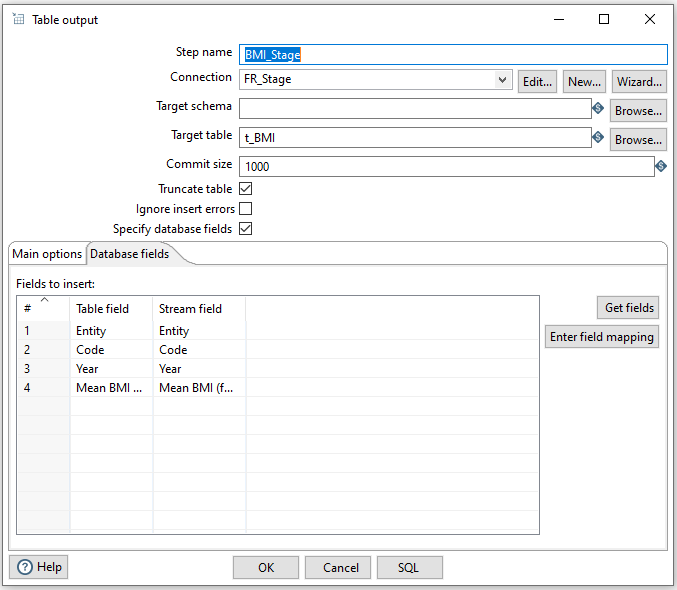
\includegraphics[width=\textwidth]{DP-obrazky/table_output.png}
    \caption{Ukázka nastavení v Table output.}
    \label{fig:Table_output}
\end{figure}

Následně stačí přidat tuto transakci do Stage jobu, aby bylo možné vše automatizovat. (Při vytváření je ideální si otevřít jinou stage transakci a nechat se jí inspirovat).

\begin{figure}
    \centering
    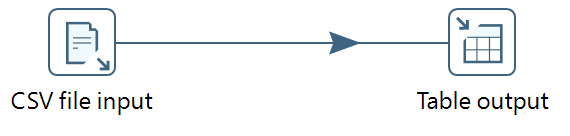
\includegraphics[width=\textwidth]{DP-obrazky/Stage_sablona.png}
    \caption{Ukázka šablony prvků pro Stage transakci.}
    \label{fig:Stage_šablona}
\end{figure}

\subsection{Vytvoření transakce pro Transform}
Nejdříve vytvoříme novou transakci a do ní vložíme \textbf{Table input}, ke kterému připojíme \textbf{Stage} databázi. Zvolíme možnost \textbf{Get SQL select statement…} Ve výběru zvolíme tabulku, z které chceme vzít data a vezmeme z ní všechny sloupce. 

\begin{figure}
    \centering
    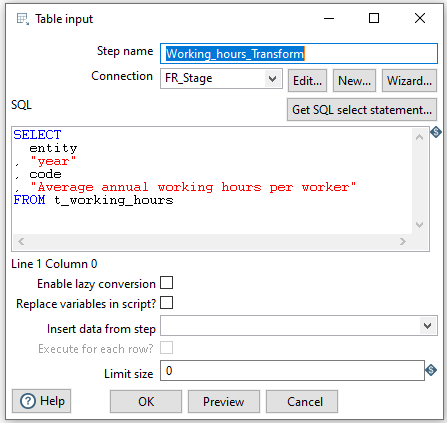
\includegraphics[width=\textwidth]{DP-obrazky/table_input.png}
    \caption{Ukázka nastavení v Table input.}
    \label{fig:Table_input}
\end{figure}

Další úpravy jsou závislé na tom, jak jsou všechny data v dané datové sestavě uložena, ale vždy je třeba zvolit \textbf{Select values}, kde všechny nepotřebné sloupce zařadíme do kolonky \textbf{Remove} a zbylé sloupce přejmenujeme dle následné šablony:

\begin{description}
    \item[country] - sloupec pro název země
    \item[date] - sloupec pro časový údaj ve tvaru yyyy a formátu int
    \item[value] - sloupec pro vlastní hodnotu měřené veličiny
\end{description}


\begin{figure}
    \centering
    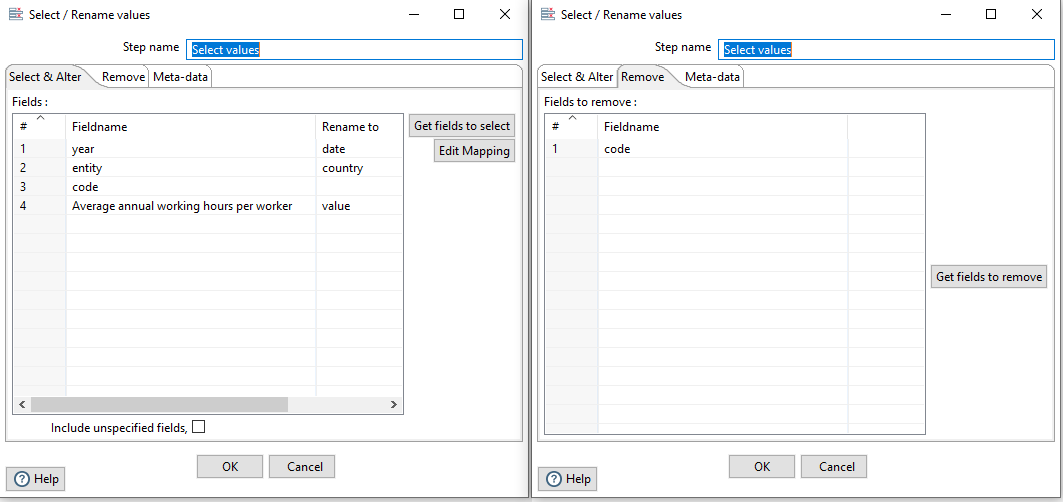
\includegraphics[width=\textwidth]{DP-obrazky/select_values.png}
    \caption{Ukázka nastavení v Select values a Remove.}
    \label{fig:Select_vals}
\end{figure}

Poslední nutnou úpravou je uložená tohoto datového souboru do CSV do složky \textbf{transform}, z níž budou všechny CSV soubory transformovány pomocí Python skriptu \textbf{data\_transform.py}, který upraví názvy zemí, aby byly jednotné, a otestuje stacionaritu dat.

K tomu je potřeba přidat \textbf{Text file output}. V něm zvolit na úvodní stránce správnou cestu, kam se má soubor uložit (\${path}\textbackslash DP-data\textbackslash transform\textbackslash + náš název souboru bez přípony). V \textbf{Extension} zvolíte csv. 

V části \textbf{Content} zvolíte jako Separator ; a jako Enclosure “. Potvrdíte Header a pokračujete na kolonku \textbf{Fields}, kde opět přes \textbf{Get Fields} dostanete obsah a následně zvolíte možnost \textbf{Minimal width}, aby se nuceně neroztahovaly stringy.

\begin{figure}
    \centering
    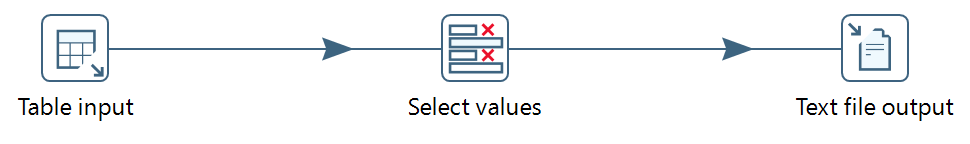
\includegraphics[width=\textwidth]{DP-obrazky/transform_sablona.png}
    \caption{Ukázka šablony prvků pro Transform transakci.}
    \label{fig:Transform_šablona}
\end{figure}

Výsledek je následně uložen do souboru \textbf{Converted\_Data\_Sources}, z něhož se následně načítají data v dalším kroku. Po dokončení je třeba tuto transformaci přidat do \textbf{Transform} Pentaho Jobu, aby byl tento krok zařazen do automatizovaného procesu tvorby datového skladu.

\subsection{Vytvoření transakce pro Target}
Opět je třeba nejdříve vytvořit transakci, v níž zvolíte \textbf{CSV file input}, kde vybereme náš transformovaný soubor z \textbf{Converted\_Data\_Sources}. Pokud tento soubor ještě nemáme transformovaný, pouze vytvoříme cestu, kde se bude nacházet a samotné sloupce doplníme dle šablony z jiné Target transakce, neboť v této fázi mají již všechny soubory jednotný tvar.
Nastavení této položky je stejné, jako v případě části pro Stage. Jen je potřeba do první kolonky vložit název \textbf{ID}ID, protože ten není obsažen v headeru CSV souboru.

Dále je potřeba přidat sloupec \textbf{Name} s názvem proměnné, což lze provést možností \textbf{Add constants}, v níž zvolíme  \textbf{Type string} a \textbf{Value} dle názvu naší proměnné. I když by to nemělo být již třeba, lze provést další nezbytné úpravy, aby následná data odpovídala tabulce \textbf{t\_correlants} bez pomocných sloupců.

\begin{figure}
    \centering
    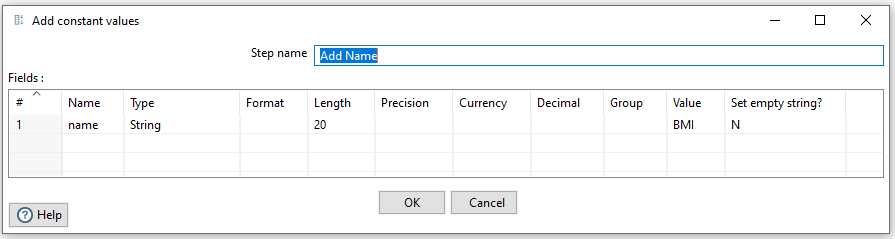
\includegraphics[width=\textwidth]{DP-obrazky/add_value.png}
    \caption{Ukázka nastavení v add constants pro přidaní sloupce Name.}
    \label{fig:Add_constants}
\end{figure}

Následně přidejte z toolboxu \textbf{Dimension lookup/update}, kde je opět třeba připojit nyní \textbf{Target} databázi. A doplnit správně všechny parametry technických proměnných. \textbf{Key fields} by měli být vždy sloupce pro Zemi a Název proměnné (Country, Name). Type of dimensional update je \textbf{Insert} a názvy sloupců by měly odpovídat názvům v \textbf{Target} databázi a není třeba již nic upravovat.
 
\begin{figure}
    \centering
    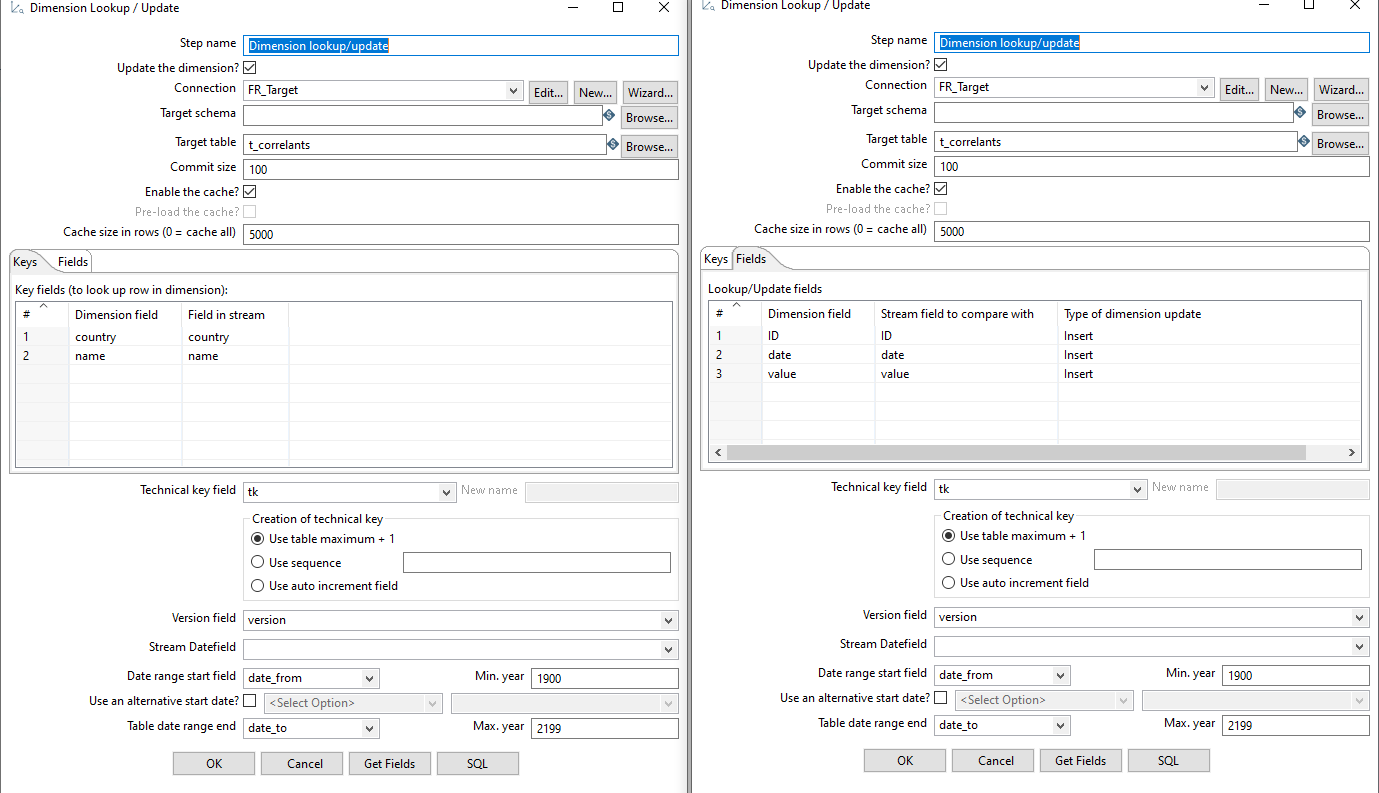
\includegraphics[width=\textwidth]{DP-obrazky/Dim_lookup.png}
    \caption{Ukázka nastavení Dimension lookup pro přidání dat do Target databáze a jejich historizaci.}
    \label{fig:Dim_Lookup}
\end{figure}
 
Následně je opět třeba přidat danou transakci do Target Jobu (FR\_Target) a je velmi vhodné postupovat dle jiné target transakce na datech podobných.

\begin{figure}
    \centering
    
\includegraphics[width=\textwidth]{DP-obrazky/target_sablona.png}
    \caption{Ukázka šablony prvků pro Target transakci.}
    \label{fig:Target_šablona}
\end{figure}

% % % % % % % % % % % % % % % % % % % % % % % % % % % % 
% % Tuto kapitolu z výsledné práce ODSTRAŇTE.
% % % % % % % % % % % % % % % % % % % % % % % % % % % % 
% 
% \chapter{Návod k~použití této šablony}
% 
% Tento dokument slouží jako základ pro napsání závěrečné práce na Fakultě informačních technologií ČVUT v~Praze.
% 
% \section{Výběr základu}
% 
% Vyberte si šablonu podle druhu práce (bakalářská, diplomová), jazyka (čeština, angličtina) a kódování (ASCII, \mbox{UTF-8}, \mbox{ISO-8859-2} neboli latin2 a nebo \mbox{Windows-1250}). 
% 
% V~české variantě naleznete šablony v~souborech pojmenovaných ve formátu práce\_kódování.tex. Typ může být:
% \begin{description}
% 	\item[BP] bakalářská práce,
% 	\item[DP] diplomová (magisterská) práce.
% \end{description}
% Kódování, ve kterém chcete psát, může být:
% \begin{description}
% 	\item[UTF-8] kódování Unicode,
% 	\item[ISO-8859-2] latin2,
% 	\item[Windows-1250] znaková sada 1250 Windows.
% \end{description}
% V~případě nejistoty ohledně kódování doporučujeme následující postup:
% \begin{enumerate}
% 	\item Otevřete šablony pro kódování UTF-8 v~editoru prostého textu, který chcete pro psaní práce použít -- pokud můžete texty s~diakritikou normálně přečíst, použijte tuto šablonu.
% 	\item V~opačném případě postupujte dále podle toho, jaký operační systém používáte:
% 	\begin{itemize}
% 		\item v~případě Windows použijte šablonu pro kódování \mbox{Windows-1250},
% 		\item jinak zkuste použít šablonu pro kódování \mbox{ISO-8859-2}.
% 	\end{itemize}
% \end{enumerate}
% 
% 
% V~anglické variantě jsou šablony pojmenované podle typu práce, možnosti jsou:
% \begin{description}
% 	\item[bachelors] bakalářská práce,
% 	\item[masters] diplomová (magisterská) práce.
% \end{description}
% 
% \section{Použití šablony}
% 
% Šablona je určena pro zpracování systémem \LaTeXe{}. Text je možné psát v~textovém editoru jako prostý text, lze však také využít specializovaný editor pro \LaTeX{}, např. Kile.
% 
% Pro získání tisknutelného výstupu z~takto vytvořeného souboru použijte příkaz \verb|pdflatex|, kterému předáte cestu k~souboru jako parametr. Vhodný editor pro \LaTeX{} toto udělá za Vás. \verb|pdfcslatex| ani \verb|cslatex| \emph{nebudou} s~těmito šablonami fungovat.
% 
% Více informací o~použití systému \LaTeX{} najdete např. v~\cite{wikilatex}.
% 
% \subsection{Typografie}
% 
% Při psaní dodržujte typografické konvence zvoleného jazyka. České \uv{uvozovky} zapisujte použitím příkazu \verb|\uv|, kterému v~parametru předáte text, jenž má být v~uvozovkách. Anglické otevírací uvozovky se v~\LaTeX{}u zadávají jako dva zpětné apostrofy, uzavírací uvozovky jako dva apostrofy. Často chybně uváděný symbol "{} (palce) nemá s~uvozovkami nic společného.
% 
% Dále je třeba zabránit zalomení řádky mezi některými slovy, v~češtině např. za jednopísmennými předložkami a spojkami (vyjma \uv{a}). To docílíte vložením pružné nezalomitelné mezery -- znakem \texttt{\textasciitilde}. V~tomto případě to není třeba dělat ručně, lze použít program \verb|vlna|.
% 
% Více o~typografii viz \cite{kobltypo}.
% 
% \subsection{Obrázky}
% 
% Pro umožnění vkládání obrázků je vhodné použít balíček \verb|graphicx|, samotné vložení se provede příkazem \verb|\includegraphics|. Takto je možné vkládat obrázky ve formátu PDF, PNG a JPEG jestliže používáte pdf\LaTeX{} nebo ve formátu EPS jestliže používáte \LaTeX{}. Doporučujeme preferovat vektorové obrázky před rastrovými (vyjma fotografií).
% 
% \subsubsection{Získání vhodného formátu}
% 
% Pro získání vektorových formátů PDF nebo EPS z~jiných lze použít některý z~vektorových grafických editorů. Pro převod rastrového obrázku na vektorový lze použít rasterizaci, kterou mnohé editory zvládají (např. Inkscape). Pro konverze lze použít též nástroje pro dávkové zpracování běžně dodávané s~\LaTeX{}em, např. \verb|epstopdf|.
% 
% \subsubsection{Plovoucí prostředí}
% 
% Příkazem \verb|\includegraphics| lze obrázky vkládat přímo, doporučujeme však použít plovoucí prostředí, konkrétně \verb|figure|. Například obrázek \ref{fig:float} byl vložen tímto způsobem. Vůbec přitom nevadí, když je obrázek umístěn jinde, než bylo původně zamýšleno -- je tomu tak hlavně kvůli dodržení typografických konvencí. Namísto vynucování konkrétní pozice obrázku doporučujeme používat odkazování z~textu (dvojice příkazů \verb|\label| a \verb|\ref|).
% 
% \begin{figure}\centering
% 	
\includegraphics[width=0.5\textwidth, angle=30]{cvut-logo-bw}
% 	\caption[Příklad obrázku]{Ukázkový obrázek v~plovoucím prostředí}\label{fig:float}
% \end{figure}
% 
% \subsubsection{Verze obrázků}
% 
% % Gnuplot BW i barevně
% Může se hodit mít více verzí stejného obrázku, např. pro barevný či černobílý tisk a nebo pro prezentaci. S~pomocí některých nástrojů na generování grafiky je to snadné.
% 
% Máte-li například graf vytvořený v programu Gnuplot, můžete jeho černobílou variantu (viz obr. \ref{fig:gnuplot-bw}) vytvořit parametrem \verb|monochrome dashed| příkazu \verb|set term|. Barevnou variantu (viz obr. \ref{fig:gnuplot-col}) vhodnou na prezentace lze vytvořit parametrem \verb|colour solid|.
% 
% \begin{figure}\centering
% 	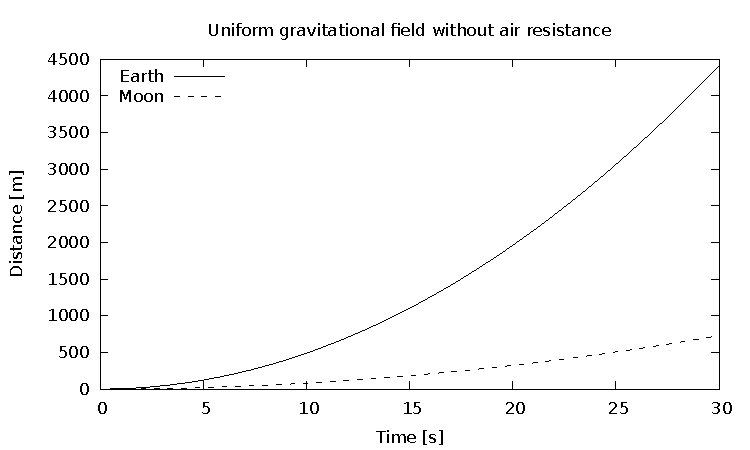
\includegraphics{gnuplot-bw}
% 	\caption{Černobílá varianta obrázku generovaného programem Gnuplot}\label{fig:gnuplot-bw}
% \end{figure}
% 
% \begin{figure}\centering
% 	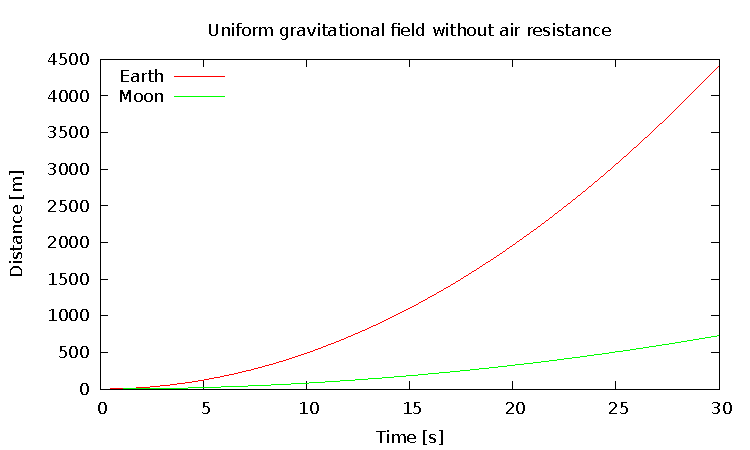
\includegraphics{gnuplot-col}
% 	\caption{Barevná varianta obrázku generovaného programem Gnuplot}\label{fig:gnuplot-col}
% \end{figure}
% 
% 
% \subsection{Tabulky}
% 
% Tabulky lze zadávat různě, např. v~prostředí \verb|tabular|, avšak pro jejich vkládání platí to samé, co pro obrázky -- použijte plovoucí prostředí, v~tomto případě \verb|table|. Například tabulka \ref{tab:matematika} byla vložena tímto způsobem.
% 
% \begin{table}\centering
% 	\caption[Příklad tabulky]{Zadávání matematiky}\label{tab:matematika}
% 	\begin{tabular}{|l|l|c|c|}\hline
% 		Typ		& Prostředí		& \LaTeX{}ovská zkratka	& \TeX{}ovská zkratka	\tabularnewline \hline \hline
% 		Text		& \verb|math|		& \verb|\(...\)|	& \verb|$...$|		\tabularnewline \hline
% 		Displayed	& \verb|displaymath|	& \verb|\[...\]|	& \verb|$$...$$|	\tabularnewline \hline
% 	\end{tabular}
% \end{table}
% 
% % % % % % % % % % % % % % % % % % % % % % % % % % % % 

\chapter{Obsah přiloženého CD}

%upravte podle skutecnosti

\begin{figure}
	\dirtree{%
	    .1 readme.txt\DTcomment{stručný popis obsahu}.
		.1 FR\_Dashboard\DTcomment{Power BI dashboard s data použitá v této práci}.
		.1 DP-data.
		.2 Original\_Data\_Sources\DTcomment{originální datové sady}.
	    .2 Google\_Trans\DTcomment{dílčí části datových sad stažených z Google trends}.
	    .2 transform\DTcomment{pomocné soubory sloužící pro následnou transformaci}.
	    .2 Converted\_Data\_Sources\DTcomment{transformovaná data}.
	    .2 Pictures\DTcomment{obrázky modelů, grafů a teoretických ukázek}.
	    .2 Python\_scripts\DTcomment{python skripty}.
	    .2 SQL\DTcomment{SQL soubory pro vytvoření datového skladu}.
	    .2 Pentaho\_Transactions\DTcomment{zdrojové kódy pro pentaho transakce}.
	    .2 Pentaho\_Jobs\DTcomment{zdrojové kódy pro pentaho joby}.
	    .2 DP-TFR\DTcomment{zdrojový kód pro Enterprase Architect}.
	    .1 thesis.
	    .2 thesis\_latex\DTcomment{zdrojová data práce ve formatu \LaTeX}.
	    .2 thesis.pdf\DTcomment{text práce ve formátu PDF}.
	    	}
\end{figure}

\end{document}
